%\newpage 

\appendix
%\addtocontents{toc}{\protect\setcounter{tocdepth}{-1}}
\section{Proofs of some deterministic estimates}

This appendix is devoted to proving several deterministic estimates used in the main proof.

\subsection{Proof of \texorpdfstring{\Cref{lem_propTH}}{DeterLemma}}\label{sec:pf_propTH}

 
%\begin{proof}[Proof of Lemma \ref{lem_propTH}]\label{sec:pf_propTH}

Property 1 follows from the underlying symmetry of $S^{(\sB)}$ in the random band matrix model, where $M^{(\sig_1,\sig_2)}$ is a scalar matrix, or from the symmetry of $M^{(\sig_1,\sig_2)}$ in the block Anderson model, where \smash{$S^{(\sB)}$} is the identity matrix. Property 2 is a consequence of the translation invariance of the matrix $M^{(\sig_1,\sig_2)}S^{(\sB)}$. Property 3 follows from the fact that \smash{$\Theta^{(\sig_1,\sig_2)}_t$} is a rational function of $S^{(\sB)}$ in the random band matrix model, and from the fact that $S^{(\sB)}=I_{L^d}$ in the block Anderson model. 
To prove property 4, we expand \smash{$\Theta^{(\sig_1,\sig_2)}_t$} using the Taylor series
\be\label{eq;Taylor}
\Theta^{(\sig_1,\sig_2)}_t= \sum_{k=0}^\infty   t^k \big(M^{(\sig_1,\sig_2)}S^{(\sB)}\big)^k.\ee
Since $|M_{ab}^{(\sig_1,\sig_2)}|\le M_{ab}^{(+,-)}$ for both models, it follows that for any $\sig_1,\sig_2\in\{+,-\}$,
\[ |\Theta_{t,ab}^{(\sig_1,\sig_2)}| \le  \sum_{k=0}^\infty t^k \big(M^{(+,-)}S^{(\sB)}\big)_{ab}^k  = \Theta_{t,ab}^{(+,-)}.\]
The estimate \eqref{eq:THETAinftinf} then follows directly from this inequality and the identity $\sum_{b}\Theta_{t,ab}^{(+,-)}\equiv (1-t)^{-1}$, which holds because \smash{$M^{(+,-)}S^{(\sB)}$} is doubly stochastic. This uses $|m|=1$ in the random band matrix model, and Ward's identity \eqref{eq:WardM} in the block Anderson model. 


To prove \eqref{prop:ThfadC_short} for the random band matrix model, we use the following shifted Taylor expansion:
\be\label{eq:shiftTaylor} \Theta_t^{(+,+)} = \frac{1}{1+\e}\sum_{k=0}^\infty \p{\frac{t m^2 S^{(\sB)} + \e}{1+\e}}^k, \ee
where $\e>0$ is a positive constant. As shown in \cite[Lemma 4.2]{bourgade2019random}, one has $\|(tm^2 S^{(\sB)} + \e)/(1+\e)\|_{\infty\to \infty} \le 1-c$ for some constant $c>0$ depending on $\e$ and $\kappa$. Applying this estimate to the expansion \eqref{eq:shiftTaylor} and noticing that the off-diagonal entries of $\p{t m^2 S^{(\sB)} + \e}/\p{1+\e}$ contain a $\ilambda^2$ factor (by the definition \eqref{eq:variancematrix}), we derive the bound \eqref{prop:ThfadC_short}. For the block Anderson model, we instead use the Taylor expansion % for $\sig_1=\sig_2=+$:
\begin{align}
\left(1-tM^{(+,+)}\right)^{-1}_{0a} &=\left[\left(1-tm^2\right)I - t M'\right]^{-1}_{0a} = \sum_{k=0}^{\infty}\left(1-tm^2\right)^{-(k+1)}
 \left(t M'\right)^{k}_{0a},\label{eq:expMLn}
\end{align}
where $M':=M^{(+,+)}- m^2I$ is obtained from $M^{(+,+)}$ by setting its diagonal entries to zero.
By property (2) of \Cref{lem:propM}, there exists a constant $\e>0$ such that $|1-tm^2|\ge \e$ and
\be\label{eq:off_diagM}
\|M'\|_{\infty\to \infty}= \sum_{a\ne 0}|M'_{0a}| = 1 - |m|^2 \le (1-\e)|1-tm^2| ,\quad \forall t\in[0,1].
\ee
Applying this bound to \eqref{eq:expMLn}, we deduce the following estimate: there exists a constant $C>0$ such that for any $\delta>0$,
\begin{align}
\Big|\big(1-tM^{(+,+)}\big)^{-1}_{0a}\Big| &\le  \sum_{0\le k\le \delta |a|}\left(1-tm^2\right)^{-(k+1)}
 \left(t M'\right)^{k}_{0a} + \e^{-1}\sum_{k> \delta |a|}(1-\e)^k \nonumber\\
&\le \sum_{0\le k\le \delta |a|} C^k \exp(-c|a|) +\e^{-2}(1-\e)^{\delta|a|} \le C' e^{-c' |a|}.\label{eq:expMLn2}
\end{align}
In the second inequality, we use the exponential decay of $M'$ by \eqref{Mbound_AO} or \eqref{Mbound_AO2}, together with the convolution bound $\sum_{b}e^{-c|a_1-b|-c|a_2-b|}\lesssim e^{-c|a_1-a_2|}$ for all $a_1,a_2\in \Zn$, and in the third inequality we choose $\delta>0$ sufficiently small so that $C^{\delta}\le e^{c/2}$. The constants $c', C'$ depend only on $C,\ c,\ \e$, and $\delta$. The bound \eqref{eq:expMLn2} yields \eqref{prop:ThfadC_short} in the regime $\ilambda\gtrsim 1$. When $\ilambda\ll 1$, we return to \eqref{eq:expMLn} and note that $\|M'\|_{\infty\to\infty}\lesssim \ilambda^2$ by \eqref{Mbound_AO}. In this case, for $a\ne 0$, the same argument as in \eqref{eq:expMLn2} applies, leading to the bound \eqref{prop:ThfadC_short}.


% When $\ilambda\ll 1$, using \eqref{eq:expMLn} and $\|M'\|_{\infty\to\infty}\lesssim \lambda^2$ by \eqref{Mbound_AO}, we can derive \eqref{prop:ThfadC_short} for the case $a\ne 0$ with a similar argument as in \eqref{eq:expMLn2}. 

%\eqref{Mbound_AO} and \eqref{Mbound_AO2}, we have that \smash{$|1-tM^{(+,+)}_{00}|\gtrsim 1$} and $\|M'\|\lesssim \lambda^2$. Applying them to \eqref{eq:expMLn} and recalling that $S^{(\sB)}=I$, we can  conclude \eqref{prop:ThfadC_short}.

%The bounds \eqref{prop:BD1}--\eqref{prop:ThfadC0} are immediate consequences of \eqref{prop:ThfadC_short} when $\sig_1=\sig_2$. It remains to handle the case $\sig_1\ne \sig_2$. In this case, the bounds \eqref{prop:ThfadC0} and \eqref{prop:BD2} were established in \cite{yang2024Del} by analyzing the Fourier series of \smash{$\zTheta_t^{(+,-)}$} via a standard summation-by-parts argument.\footnote{In \cite{yang2024Del}, the assumption $\ilambda\ll 1$ was imposed; but essentially the same (and actually slightly easier) argument applies to the case $\ilambda\gtrsim 1$.} 

The bounds \eqref{prop:ThfadC} and \eqref{prop:BD1}--\eqref{prop:ThfadC0} follow directly from \eqref{prop:ThfadC_short} in the case $\sigma_1=\sigma_2$. It therefore remains to consider the case $\sigma_1\neq \sigma_2$. In this case, the estimates \eqref{prop:ThfadC0} and \eqref{prop:BD2} were proved in \cite{yang2024Del} by analyzing the Fourier series of \smash{$\zTheta_t^{(+,-)}$} through a standard summation-by-parts argument.\footnote{In \cite{yang2024Del}, the assumption $\ilambda\ll 1$ was imposed; however, the same argument (in fact, slightly simpler) applies when $\ilambda\gtrsim 1$.} 
Specifically, \eqref{prop:ThfadC0} is proved in Lemma 3.1 of \cite{yang2024Del}, while \eqref{prop:BD2} appears as equation (E.19) therein. Although the bound \eqref{prop:BD1} is not stated explicitly in \cite{yang2024Del}, its proof proceeds analogously to those of \eqref{prop:ThfadC0} and \eqref{prop:BD2}, by applying the same summation-by-parts technique to the corresponding Fourier expansion. We therefore omit the details.
These bounds \eqref{prop:BD1}--\eqref{prop:ThfadC0} have also been derived for dimension $d=2$ in \cite[Lemma 3.10]{RBSO1D}, where the summation-by-parts argument is explained in Appendix~B. The same reasoning extends directly to dimensions $d\ge 3$.
 

%More precisely, \eqref{prop:ThfadC0} is proved in Lemma 3.1 of \cite{yang2024Del}, while \eqref{prop:BD2} is proved as (E.19) in \cite{yang2024Del}. Although the estimate \eqref{prop:BD1} does not appear explicitly in \cite{yang2024Del}, its proof is similar to those for \eqref{prop:ThfadC0} and \eqref{prop:BD2} by estimating the related Fourier series using the same summation by parts argument. Hence, we omit the details of the proof. 


Finally, it remains to prove the bound \eqref{prop:ThfadC} for the case $\sig_1\ne \sig_2$. Its proof is similar to that of \cite[Lemma 2.14]{DYYY25}, using the Taylor expansion, along with the random walk representation of \smash{$(S^{(\sB)})^k$} (for the random band matrix model), or \smash{$(M^{(+,-)})^k$} (for the block Anderson model). 
More precisely, for the random band matrix model, we consider the random walk $\{X_k:k\ge 0\}$ on $\Z^d$, with transition probabilities \smash{$\big\{p(0,a)=S_{0a}^{(\sB)}:a\in \Z^d\big\}$}.  
First, given any $a\in \Z^d\setminus\{0\}$, by applying the Bernstein inequality to $X_k\cdot \wh a$ with $\wh a$ denoting the unit vector $a/\|a\|_2$, we can derive the following large deviation estimate: there exist constants $c, C>0$ (which do not depend on $a$) such that 
\[ \P_0(X_k=a) \le C\exp\p{-c \p{\frac{|a|^2}{\ilambda^2k}\wedge |a|}},\quad \forall a\in \Z^d,\ k\ge 1 . \]
On the other hand, using the local CLT for $X_k$ (see e.g., \cite[Section 2]{Lawler_book}), we obtain that 
\[ \P_0(X_k=a) \le 1\wedge \p{C (\ilambda^2k)^{-d/2}},\quad \forall a\in \Z^d,\ k\ge 1 . \]
Combining the above two bounds and using the argument below equation (8.3) of \cite{DYYY25}, we obtain the large deviation bound
\[ \P_0(X_k=a) \le C\p{ (\ilambda^2k)^{-d/2}\wedge 1}\exp\p{-c \p{\frac{|a|^2}{\ilambda^2k}\wedge |a|}},\quad \forall a\in \Z^d,\ k\ge 1,  \]
for some constants $c,C>0$. Projecting the random walk onto the torus $\Zn$, i.e., summing this bound over the periodic images of $a$, we obtain that
\begin{equation*}\label{eq:heat_torus}\tag{$\star$}
\big(M^{(+,-)}S^{(\sB)}\big)_{0a}^k \le C\p{ (\ilambda^2k)^{-d/2}\wedge 1+L^{-d}}\exp\p{-c \p{\frac{|a|^2}{\ilambda^2k}\wedge |a|}},\quad \forall a\in \Zn,\ k\ge 1,
\end{equation*}
for some constants $c,C>0$ that do not depend on $L$. 

For the block Anderson model, the matrix $P:=M^{(+,-)}S^{(\sB)}=M^{(+,-)}$, $P_{ab}=|M^{(\sB)}_{ab}|^2$, is symmetric, translation invariant, and doubly stochastic by properties (1) and (2) of \Cref{lem:propM}; in particular, $P_{0,-a}=P_{a0}=P_{0a}$. However, $P$ depends on $L$ and $m$, and it is not the periodization of a fixed transition kernel on $\Z^d$, so the above projection argument and the local CLT do not apply. Instead, we prove \eqref{eq:heat_torus} directly on the torus, with constants $c,C>0$ depending only on $d$, $\kappa$, and $\fd$. For $x\in \Zn$ and $j\in\qqq{d}$, let $|x_j|_L$ denote the periodic distance between the $j$-th coordinate of $x$ and $0$, so that $|x|=\max_j|x_j|_L$. 

\smallskip
\noindent{\it Step 1: Fourier symbol.} The eigenvalues of $\Psi^{(\sB)}$ are $\psi_q:=2\sum_{j=1}^d\cos q_j$, $q\in (\Zn)^*:=(2\pi/L)\Zn\subset(-\pi,\pi]^d$, with eigenvectors $(L^{-d/2}e^{\ii q\cdot a})_{a\in\Zn}$. Hence, setting $f_q:=(\ilambda\psi_q-E-m)^{-1}$, we have $M^{(\sB)}_{0a}=L^{-d}\sum_{q\in(\Zn)^*}f_qe^{-\ii q\cdot a}$, and Ward's identity \eqref{eq:WardM} reads $L^{-d}\sum_q|f_q|^2=1$. In particular, $|f_q|\ge 1$ for some $q$, which gives $|E|\le 2d\ilambda+2$ (recall $|m|\le 1$), and therefore $|f_q|\ge R^{-1}$ for all $q$, where $R:=4d\ilambda+3\lesssim 1$. The Fourier transform of $P_{0\cdot}$ is 
\[\wh P(p):=\sum_{a\in\Zn}P_{0a}e^{-\ii p\cdot a}=\frac{1}{L^d}\sum_{q\in(\Zn)^*} f_q\overline{f_{q+p}},\qquad p\in(\Zn)^*,\]
which is real since $P_{0,-a}=P_{0a}$. Using $L^{-d}\sum_q|f_q|^2=1$, $f_{q+p}-f_q=\ilambda(\psi_q-\psi_{q+p})f_qf_{q+p}$, and $L\ge 3$, we obtain that
\[1-\wh P(p)=\frac{1}{2L^d}\sum_q|f_{q+p}-f_q|^2\ge \frac{\ilambda^2}{2R^4}\cdot\frac{1}{L^d}\sum_q(\psi_{q+p}-\psi_q)^2=\frac{2\ilambda^2}{R^4}\sum_{j=1}^d(1-\cos p_j).\]
On the other hand, $1+\wh P(p)=\sum_a P_{0a}(1+\cos(p\cdot a))\ge 2P_{00}=2|m|^2\ge 2(\im m)^2\gtrsim 1$ by property (2) of \Cref{lem:propM}. Since $\ilambda\le\fd^{-1}$, these two bounds yield that, for a constant $c_1>0$,
\[
|\wh P(p)|\le 1-c_1\ilambda^2|p|^2,\quad \forall p\in (\Zn)^*.
\]

\smallskip
\noindent{\it Step 2: on-diagonal bound.} By Fourier inversion and the bound in Step 1, $P^{2k}_{00}=L^{-d}\sum_{p}\wh P(p)^{2k}\le L^{-d}\sum_{p}e^{-2c_1k\ilambda^2|p|^2}\le C\big((\ilambda^2k)^{-d/2}+L^{-d}\big)$, where the term $L^{-d}$ comes from $p=0$. Moreover, by the Cauchy--Schwarz inequality, the symmetry and the translation invariance of $P$, we have $P^{2k}_{0a}=\sum_bP^k_{0b}P^k_{ba}\le (P^{2k}_{00}P^{2k}_{aa})^{1/2}=P^{2k}_{00}$ and $P^{2k+1}_{0a}=\sum_bP_{0b}P^{2k}_{ba}\le P^{2k}_{00}$. Together with $P^k_{0a}\le 1$, this gives
\[
\max_{a}P^k_{0a}\le C\p{(\ilambda^2k)^{-d/2}\wedge 1+L^{-d}},\quad \forall k\ge 1. 
\]

\smallskip
\noindent{\it Step 3: tail bound.} Fix $j\in\qqq{d}$ and $\mu\ge 0$, and let $F_\mu(x):=\cosh(\mu|x_j|_L)$. For $x,y\in\Zn$, choose integer representatives $\wt x_j,\wt y_j$ of $x_j,y_j$ with $|\wt x_j|=|x_j|_L$ and $|\wt y_j|=|y_j|_L$. Since $|x_j\pm y_j|_L\le |\wt x_j\pm \wt y_j|$, we have $F_\mu(x+y)+F_\mu(x-y)\le 2F_\mu(x)\cosh(\mu |y_j|_L)$. Together with $P_{0,-y}=P_{0y}$, this implies
\[(PF_\mu)(x)=\frac12\sum_y P_{0y}\big(F_\mu(x+y)+F_\mu(x-y)\big)\le F_\mu(x)\sum_y P_{0y}\cosh(\mu|y|)\le \p{1+C\ilambda^2\mu^2}F_\mu(x),\quad \forall\, 0\le\mu\le c,\]
where in the last step we used $\sum_{y\ne 0}P_{0y}|y|^2e^{2c|y|}\le C\ilambda^2$, which follows from \eqref{Mbound_AO} when $\ilambda<(2C)^{-1}$ and from \eqref{Mbound_AO2} when $\ilambda\ge (2C)^{-1}$. Iterating this bound and applying the exponential Chebyshev inequality, we get $\sum_{x:|x_j|_L\ge r}P^k_{0x}\le e^{C\ilambda^2\mu^2k}/\cosh(\mu r)$ for all $r\ge 0$. Optimizing over $\mu\in[0,c]$ and taking a union bound over $j\in\qqq{d}$, we obtain that
\[
\sum_{x:|x|\ge r}P^k_{0x}\le 2d\exp\p{-c\p{\frac{r^2}{\ilambda^2k}\wedge r}},\quad \forall r\ge 0,\ k\ge 1.
\]

\smallskip
\noindent{\it Step 4: conclusion.} For $k\ge 2$, write $k=k_1+k_2$ with $k_1=\lceil k/2\rceil$ and $k_2=\lfloor k/2\rfloor$. Since $|b|\ge |a|/2$ or $|a-b|\ge |a|/2$ for every $b\in\Zn$, we have
\[P^k_{0a}=\sum_b P^{k_1}_{0b}P^{k_2}_{ba}\le \max_{x}P^{k_2}_{0x}\sum_{b:|b|\ge |a|/2}P^{k_1}_{0b}+\max_xP^{k_1}_{0x}\sum_{b:|b-a|\ge|a|/2}P^{k_2}_{ab}.\]
Applying the bounds of Steps 2 and 3 to the right-hand side yields \eqref{eq:heat_torus} for $k\ge 2$, while the case $k=1$ follows directly from \eqref{Mbound_AO} and \eqref{Mbound_AO2}. 

\smallskip
Finally, for both models, applying \eqref{eq:heat_torus} to the expansion \eqref{eq;Taylor} and summing over $k$, we can derive the desired bound \eqref{prop:ThfadC}.
Since the argument closely follows that in \cite[Section 8]{DYYY25}, we omit the details. In fact, the proof here is somewhat simpler than in \cite{DYYY25}, because $d=2$ is the critical dimension, where logarithmic corrections (e.g., $\log L$) appear. In contrast, for $d\ge 3$, all relevant series (or integrals) are summable, resulting in a dimension-dependent constant $C_d$ in \eqref{prop:ThfadC}.


%\end{proof}

%With this bound, we can control $(S^{(\sB)})_{0a}^k$ by projecting this random walk onto the torus $\Zn$. Then, summing over these estimates and using \eqref{eq;Taylor}, we can derive the bound \eqref{prop:ThfadC}. Since the argument is similar to that in \cite{DYYY25}, we omit the details. In fact, the proof here is relatively easier than that in \cite{DYYY25}, because $d=2$ is the critical dimension where some $\log L$ factors would appear. On the other hand, for dimensions $d\ge 3$, all related series are summable, which leads to the constant $C_d$ in \eqref{prop:ThfadC}. 

%{The proof of Lemma \ref{lem_propTH} is based on the random walk representation and pointwise estimates for $(S^{(B)})^{k}$ that agree with the continuum Gaussian heat kernel estimates. A proof is given in Section \ref{sec_TH}; the argument is long and elementary, so we give an intuitive explanation of Lemma \ref{lem_propTH} below.

% The first four properties in Lemma \ref{lem_propTH} are standard. For the exponential decay \eqref{prop:ThfadC} for the discrete Laplacian on $\Z^{2}$ (instead of $S^{(B)}-\mathrm{Id}$) can be found in Theorem 1.3 of \cite{MS22} (see also the discussion following it therein). The difference between the full space $\Z^{2}$ and the torus $\Z_{L}^{2}$ is that if $\ell_t=L$, so that $|1-t|^{-1/2}\geq L$, then the periodic boundary conditions on $\Z_{L}^{2}$ automatically introduces a space-cutoff of scale $L$ (before the cutoff at scale $|1-t|^{-1/2}$ that is imposed by the resolvent). One can also check that \eqref{prop:ThfadC} implies 
% \begin{align*}
% \sum_{b\in\Z_{L}^{2}}(\Theta^{(B)}_{\xi})_{ab}\prec|1-t|^{-1},
% \end{align*}
% which can be checked using the random walk representation as well. 


%The gradient bounds \eqref{prop:BD1}-\eqref{prop:BD2} are standard, in that the Green's function for the Laplacian on $\R^{2}$ is $\log|x|$. Thus, the first terms on the right-hand side of \eqref{prop:BD1}-\eqref{prop:BD2} agree with its derivatives. (The support-length of the gradients is also of order $\ell_t$, but we will not need this fact.) The additional corrections come from the periodic boundary of $\Z_{L}^{2}$. The scaling of the last term in \eqref{prop:BD2} agrees with the heuristic that $\Theta^{(B)}$ is the resolvent for the diffusion of a generator, so its second-derivative should have $L^{1}$ norm of size $\mathrm{O}_{\prec}(1)$. The last term in \eqref{prop:BD1} therefore interpolates between \eqref{prop:ThfadC} and the last term in \eqref{prop:BD2}.}
\subsection{Proofs of evolution kernel estimates}\label{ks}

In this subsection, we present the proofs of \Cref{lem:sum_Ndecay,lem:sum_decay,lem:sum_decay_nonzero}. 
% During the main proof, we rely on several estimates for the evolution kernel (defined in \Cref{DefTHUST}), which are stated in this section and used to control the terms in \eqref{int_K-LcalE}. 
Parts of the proofs parallel those in \cite{YY_25,DYYY25,RBSO1D} for random band matrices and for the block Anderson model in dimensions 1 and 2. However, certain key arguments must be adapted to handle the higher-dimensional setting $d \ge 3$. We therefore outline the proofs of the evolution kernel estimates, emphasizing the modifications needed compared to the arguments in \cite{YY_25,DYYY25,RBSO1D}. 
%We first have an easy bound on the $({\infty\to \infty})$-norm of $\mathcal U^{(n)}_{t,\bsig,\ba}$. 

 % \begin{lemma}\label{lem:sum_Ndecay}
	%  	Let ${\cal A}: (\Zn)^{n}\to \mathbb C$ be an $n$-dimensional tensor for a fixed $n\in \N$ with $n\ge 2$. Then, for each $0\le s \le t < 1$, we have that 
	%  	\begin{align}\label{sum_res_Ndecay}
	% 	 		\| {\cal U}^{(n)}_{s,t,\bsig}\;\circ {\cal A}\|_{\infty} \le \left(  \frac{1-s}{1-t}\right)^{n }\cdot \|{\cal A}\|_{\infty} , 
	% 	 	\end{align}
	%  	where the $L^\infty$-norm of ${\cal A}$ is defined as $\|{\cal A}\|_{\infty}=\max_{\ba\in (\Zn)^n}|\cal A_{\ba}|$.
	%  \end{lemma}
\begin{proof}[\bf Proof of \Cref{lem:sum_Ndecay}]
	Notice the following decomposition:
	\be\label{eq:decompUalt}\frac{1 - s \cdot M^{(\sig_i,\sig_{i+1})}S^{(\sB)}}{1 - t \cdot M^{(\sig_i,\sig_{i+1})}S^{(\sB)}} =1+ \Xi^{(i)},\quad \text{where}\quad \Xi^{(i)}:=(t-s)\cdot M^{(\sig_i,\sig_{i+1})}S^{(\sB)} \Theta_{t}^{(\sig_i,\sig_{i+1})} .\ee
	Using \eqref{eq:THETAinftinf}, along with \eqref{eq:WardM} in the case of block Anderson model, we obtain that
	\be\label{Xi_infint} \|\Xi^{(i)}\|_{\infty\to \infty} = \max_{a}\sum_b |\Xi^{(i)}_{ab}| \le \p{t-s}\|\Theta^{(\sig_i,\sig_{i+1})}_{t}\|_{\infty\to \infty} \le \frac{t-s}{1-t}. \ee
	Together with \eqref{eq:decompUalt}, this implies that 
	$$\left\|\frac{1 - s \cdot M^{(\sig_i,\sig_{i+1})}S^{(\sB)}}{1 - t \cdot M^{(\sig_i,\sig_{i+1})}S^{(\sB)}}\right\|_{\infty\to \infty}\le \frac{1-s}{1-t} .$$
	With this estimate, we conclude \eqref{sum_res_Ndecay} immediately using the definition \eqref{def_Ustz}. 
	\end{proof}


\begin{proof}[\bf Proof of \Cref{lem:sum_decay}]
With the decomposition \eqref{eq:decompUalt}, we can express \smash{$\mathcal{U}^{(n)}_{s, t, \bsig} \circ \mathcal{A}$} as
\begin{align}\label{eq:decomp_U2}
      \left(\mathcal{U}^{(n)}_{s, t, \bsig} \circ \mathcal{A}\right)_{\ba}&=\sum_{\mathbf b\in (\Zn)^n} \prod_{i=1}^n \left( \delta_{a_ib_i}+\Xi^{(i)}_{a_ib_i} \right)  \cdot \mathcal{A}_{\mathbf b} =\sum_{\mathbf b\in (\Zn)^n}\sum_{A\subset \qqq{n}} \prod_{i\in A} \delta_{a_ib_i} \cdot \prod_{i\in A^c} \Xi^{(i)}_{a_ib_i}  \cdot \mathcal{A}_{\mathbf{b}}\, .
\end{align}
By the estimate \eqref{prop:ThfadC} (along with \eqref{Mbound_AO} or \eqref{Mbound_AO2} in the case of block Anderson model), we have that
\be\label{eq:decayXi}
\Xi^{(i)}_{a_ib_i}\lesssim (1-s)\frac{(\ilambda^2+|1-t|)^{-1}}{(|a_i-b_i|+1)^{d-2}} e^{-c |a_i-b_i|/ {\ell}_t} 
\ee
for a constant $c>0$. 
%Moreover, we have the following bound by \eqref{eq:THETAinftinf} (along with \eqref{eq:WardM} in the case of block Anderson model): 
%\be\label{Xi_infint} \|\Xi^{(i)}\|_{\infty\to \infty} = \max_{a}\sum_b |\Xi^{(i)}_{ab}| \le \p{1-s}\|\Theta^{(\sig_i,\sig_{i+1})}_{t}\|_{\infty\to \infty} = \frac{1-s}{1-t}. \ee
We claim that for any subset $A$ with $|A|=k\in \qqq{1,n}$, 
\be\label{sum_res_1_red0}
\sum_{\mathbf b\in (\Zn)^n} \prod_{i\in A} \delta_{a_ib_i} \cdot \prod_{i\in A^c} \Xi^{(i)}_{a_ib_i}  \cdot \mathcal{A}_{\boldsymbol{b}} \le W^{C\e}\p{\frac{\ilambda^2+|1-s|}{\ilambda^2+|1-t|}}^{n-k} \|{\cal A}\|_{\infty}+ W^{-D+C },
\ee
for a constant $C$ that does not depend on $\e$ or $D$, while for $A= \emptyset$, we claim that 
\be\label{sum_res_1_red}
\sum_{\mathbf b\in (\Zn)^n} \prod_{i=1}^n \Xi^{(i)}_{a_ib_i}  \cdot \mathcal{A}_{\boldsymbol{b}} \le W^{C\e} \frac{\ell_t^2}{\ell_s^2}\p{\frac{\ilambda^2+|1-s|}{\ilambda^2+|1-t|}}^{n} \|{\cal A}\|_{\infty}+ W^{-D+C}.
\ee
Note that combining \eqref{sum_res_1_red0} and \eqref{sum_res_1_red} concludes the proof of \eqref{sum_res_1}.   

To show the estimate \eqref{sum_res_1_red0}, we assume that $A=\qqq{1,k}$ without loss of generality. With the notations $\mathbf a'=(a_{1},\ldots,a_{k})$ and $\mathbf b'=(b_{k+1},\ldots,b_{n})$, we can bound the LHS of \eqref{sum_res_1_red0} as 
\begin{align*}
\sum_{\mathbf b'\in (\Zn)^{n-k}} \prod_{i=k+1}^n  \Xi^{(i)}_{a_ib_i}  \cdot \mathcal{A}_{\ba',\mathbf{b}'} &\lesssim  \frac{\left(1-s\right)^{n-k}}{(\ilambda^2+|1-t|)^{n-k}} \|\cal A\|_\infty \sum_{\mathbf b'} \prod_{i=k+1}^n\frac{\mathbf 1\left(|b_i-a_1|\le W^\e\ell_s \right)}{|a_i-b_i|^{d-2}+1} +  W^{-D+(n-k)}\\
    &\lesssim (W^{2\e})^{n-k}\left( \frac{\ell_s^2|1-s|}{\ilambda^2+|1-t|} \right)^{n-k} \|\cal A\|_\infty  + W^{-D+(n-k)} \\
    & \lesssim \p{W^{2\e}\frac{\ilambda^2+|1-s|}{\ilambda^2+|1-t|}}^{n-k} \|\cal A\|_\infty  + W^{-D+(n-k)} , 
\end{align*}
where we have used \eqref{eq:decayXi}, the decay property \eqref{deccA0} for $\cal A_{\mathbf b}$, and 
\be\label{eq:1-sells2}(1-s)\ell_s^2\asymp \ilambda^2+|1-s|,\quad \text{for}\quad s\le 1-\ilambda^2/L^{2},\ee 
along with the condition $(1-t)/(1-s)\ge W^{-1}$ and the bound \eqref{Xi_infint} in getting the $W^{-D+(n-k)}$ term. This concludes \eqref{sum_res_1_red0} for any constant $C>2(n-k)$.  
% Without loss of generality, we only prove \eqref{sum_res_1_red} for $k=n$; to handle the $k<n$ case, we can apply the same argument to  
% $$\sum_{\mathbf b'\in (\Zn)^k}  \prod_{i\in A} \Xi^{(i)}_{[a_i][b_i]}  \cdot \mathcal{A}'_{\boldsymbol{b}'},$$
% where $\mathcal{A}'_{\boldsymbol{b}'}$ is the $k$-dimensional tensor obtained by setting $[b_i]=[a_i]$ for $i\in A^c$. 
For \eqref{sum_res_1_red}, with the notation $\mathbf b'=(b_{2},\ldots,b_{n})$, we get that 
\begin{align}
   \sum_{\mathbf b}\prod_{i=1}^{n} \Xi^{(i)}_{a_ib_i} \cdot \mathcal{A}_{\mathbf b} &= \sum_{\mathbf b}\prod_{i=1}^{n} \Xi^{(i)}_{a_ib_i} \cdot \mathcal{A}_{\mathbf b}\cdot  \mathbf 1\left(\max_{i\ne j}|b_i-b_j|\le W^\e\ell_s \right) + \OO\left( W^{-D+n}\right) \nonumber\\
   &\lesssim \frac{(1-s)^{n-1}}{(\ilambda^2+|1-t|)^{n-1}} \|\cal A\|_\infty \sum_{b_1} \left|\Xi^{(1)}_{a_1b_1}\right| \sum_{\mathbf b'} \prod_{i=2}^n \frac{\mathbf 1\left(|b_i-b_1|\le W^\e\ell_s \right)}{|a_i-b_i|^{d-2}+1} +  W^{-D+n} \nonumber\\
    %&\lesssim W^{2(n-1) \e }\left(\frac{\ell_s^2|1-s|}{\ilambda^2+|1-t|}\right)^{n-1} \|\cal A\|_\infty \sum_{b_1} \left|\Xi^{(1)}_{a_1b_1}\right| + W^{-D+n} \nonumber\\
    &\lesssim W^{2(n-1) \e}\frac{1-s}{1-t}\left(\frac{\ell_s^2|1-s|}{\ilambda^2+|1-t|}\right)^{n-1} \|\cal A\|_\infty + W^{-D+n} \nonumber\\
    &\lesssim  W^{2(n-1) \e}\frac{\ell_t^2}{\ell_s^2}\left(\frac{\ilambda^2+|1-s|}{\ilambda^2+|1-t|}\right)^{n} \|\cal A\|_\infty + W^{-D+n}, \label{sum_res_deriv_red}
\end{align} 
where in the first step, we use the decay property \eqref{deccA0} for $\cal A_{\mathbf b}$ and the bound \eqref{Xi_infint} (in getting the $W^{-D+n}$ term); in the second step, we apply \eqref{eq:decayXi} for $i\in\qqq{2,n}$; in the third step, we take the summation over $\mathbf b'$ and apply \eqref{Xi_infint}; in the last step, we use \eqref{eq:1-sells2} again.  This gives \eqref{sum_res_1_red} for any constant $C>2(n-1)$.  


For the estimates \eqref{sum_res_2_NAL} and \eqref{sum_res_2}, %\eqref{sum_res_2_sym}, and \eqref{sum_res_2_doublezero}, 
we notice that when $|A| \ge 1$, \eqref{sum_res_1_red0} already gives a good enough bound. 
Hence, we only need to focus on the case where $A=\emptyset$. 
First, for Case I, due to \eqref{prop:ThfadC_short}, we can use the better bound \smash{$\sum_{b_1}|\Xi^{(1)}_{a_1b_1}|=\OO(1)$} in the third step of \eqref{sum_res_deriv_red}, which leads to \eqref{sum_res_2_NAL}. 

Next, for the estimate \eqref{sum_res_2} in Case II, we need to show that
\be\label{sum_res_2_red}
\sum_{\mathbf b\in (\Zn)^n} \prod_{i=1}^n \Xi^{(i)}_{a_ib_i}  \cdot \mathcal{A}_{\boldsymbol{b}} \le W^{C_n\e}\p{\frac{\ilambda^2+|1-s|}{\ilambda^2+|1-t|}}^{n}  \|{\cal A}\|_{\infty} +W^{-D+C_n}.
\ee
It suffices to assume that $\sigma_i\ne \sigma_{i+1}$ for all $i\in \qqq{n}$. 
We decompose $\Zn$ into the following two regions:
\[S_{\mathrm{far}}:=\Big\{b\in \Zn:\min_{i\in\qqq{n}}|b-a_i|>  W^{2\e}\ell_s\Big\},\quad S_{\mathrm{near}}:=\Big\{b\in \Zn:\min_{i\in\qqq{n}}|b-a_i|\le W^{2\e}\ell_s\Big\}.\]
Following a similar argument as in \eqref{sum_res_deriv_red}, and using that \smash{$\sum_{b_1\in S_{\mathrm{near}}} |\Xi^{(1)}_{a_1b_1}|\lesssim W^{4\e}(\ilambda^2+|1-s|)/(\ilambda^2+|1-t|)$} by \eqref{eq:decayXi} and \eqref{eq:1-sells2}, we obtain
\begin{align}
\sum_{b_1\in S_{\mathrm{near}}} \sum_{\bfb'}\prod_{i=1}^{n} \Xi^{(i)}_{a_ib_i} \cdot \mathcal{A}_{\mathbf b} \lesssim W^{2(n+1) \e} \left(\frac{\ilambda^2+|1-s|}{\ilambda^2+|1-t|}\right)^{n}\|\cal A\|_\infty + W^{-D+n}. \label{sum_res_deriv_red2}
\end{align} 
It remains to control the sum over $b_1\in S_{\mathrm{far}}$. In this case, we decompose $\Xi^{(i)}$ as 
\be\nonumber \Xi^{(i)}_{a_ib_i}=\Xi^{(i)}_{a_ib_1} + \Delta \Xi^{(i)}_{a_i;b_1b_i},\quad\text{with}\quad \Delta \Xi^{(i)}_{a_i;b_1b_i}:=\Xi^{(i)}_{a_ib_i}-\Xi^{(i)}_{a_ib_1}. \ee
Then, we expand the LHS of \eqref{sum_res_2_red} as 
\begin{align} \label{eq:decompXii}
\sum_{A: A\subset \qqq{2,n}}f(A),\quad \text{with}\quad 
f(A):=\sum_{b_1\in S_{\mathrm{far}}}\sum_{\bfb'\in (\Zn)^{n-1}}\prod_{i\in A^c}  \Xi^{(i)}_{a_ib_1} \cdot \prod_{i\in A} \Delta \Xi^{(i)}_{a_i;b_1b_i}  \cdot \mathcal{A}_{\mathbf{b}}. 
\end{align}
By the sum-zero property \eqref{sumAzero}, the leading term with $A=\emptyset$ vanishes. For the remaining terms, we will use  \eqref{eq:decayXi} to control the factors \smash{$\Xi^{(i)}_{a_ib_1}$}, and apply \eqref{eq:decayXi} and \eqref{prop:BD1} (along with \eqref{Mbound_AO} or \eqref{Mbound_AO2} in the case of block Anderson model) to control the factors %\smash{$\Xi^{(i)}_{a_ib_1}$} and 
\smash{$\Delta \Xi^{(i)}_{a_i;b_1b_i}$} for $|a_i-b_1|\ge W^{2\e}\ell_s$ and $|b_i-b_1|\le W^{\e}\ell_s$:
\be\label{eq:Xibb}
\Xi^{(i)}_{a_ib_1}\lesssim \frac{W^{-(d-1)\e}}{\ell_s^d}\left(\frac{\ilambda^2+|1-s|}{\ilambda^2+|1-t|}\right),\   \Delta \Xi^{(i)}_{a_i;b_1b_i} \lesssim  \frac{1-s}{\ilambda^2+|1-t|}\frac{|b_i-b_1|}{|a_i-b_1|^{d-1}}  \prec \frac{W^{-d\e}}{\ell_s^d}\left(\frac{\ilambda^2+|1-s|}{\ilambda^2+|1-t|}\right),
\ee
where we have also used $2(d-2)\ge d-1$ and \eqref{eq:1-sells2} in the derivation. 
Without loss of generality, suppose $2\in A$. Then, using the estimates in \eqref{eq:decayXi} and \eqref{eq:Xibb}, along with the decay property \eqref{deccA0} for $\cal A$, by a similar argument as in \eqref{sum_res_deriv_red}, we can bound $f(A)$ by 
\begin{align}
f(A)&\lesssim W^{\e (n-1)} \frac{(1-s)(\ilambda^2+|1-s|)^{n-2}}{(\ilambda^2+|1-t|)^{n-1}}  \|\cal A\|_\infty 
\sum_{b_1\in S_{\mathrm{far}}} \left|\Xi^{(1)}_{a_1b_1}\right| \frac{ (W^\e\ell_s)^{d+1}}{|a_2-b_1|^{d-1}} + W^{-D+n}L^{d(n-1)}\nonumber\\
&\lesssim  W^{(n+d+1) \e }\frac{(1-s)^2\ell_s^{d+1}(\ilambda^2+|1-s|)^{n-2}}{(\ilambda^2+|1-t|)^{n}}  \|\cal A\|_\infty  
\sum_{b_1\in S_{\mathrm{far}}} \frac{\exp(-c|a_1-b_1|/\ell_t)}{|a_1-b_1|^{d-2} \cdot |a_2-b_1|^{d-1}} + W^{-D+n}L^{d(n-1)} \nonumber\\
&\lesssim  W^{(n+d+1)\e } \|\cal A\|_\infty \cdot  \frac{(1-s)^2\ell_s^{d+1}}{(W^{2\e}\ell_s)^{d-3}}\log L\cdot \frac{(\ilambda^2+|1-s|)^{n-2}}{(\ilambda^2+|1-t|)^{n}} + W^{-D+n}L^{d(n-1)} \nonumber\\
&\lesssim W^{(n+5)\e }  \p{\frac{\ilambda^2+|1-s|}{\ilambda^2+|1-t|}}^{n} \|\cal A\|_\infty+ W^{-D+n}L^{d(n-1)}. 
\label{eq:bddfA}
\end{align}
In the third step, we used the lattice sum estimate
\be\label{eq:latticesum_d3}
\sum_{b\,:\,|a_1-b|\wedge|a_2-b|> R} \frac{\exp(-c|a_1-b|/\ell_t)}{|a_1-b|^{d-2} \cdot |a_2-b|^{d-1}} \lesssim \frac{\log L}{R^{d-3}},\quad \forall\, 1\le R\le L,
\ee
which holds for every $d\ge 3$; the logarithm is needed only in the borderline case $d=3$, where the summand decays exactly like $|b|^{-d}$ and the sum over $R\le |b|\lesssim \ell_t$ is of order $\log(\ell_t/R)$. In the last step we absorbed it using $\log L\le W^{\e}$, together with \eqref{eq:1-sells2} in the form $(1-s)^2\ell_s^4\asymp(\ilambda^2+|1-s|)^2$. The error term $W^{-D+n}L^{d(n-1)}$ comes from the region where $|\cal A_{\mathbf b}|\le W^{-D}$ by \eqref{deccA0}: there, since $\Xi^{(i)}_{a_ib_1}$ does not depend on $b_i$, we have $\sum_{b_i}\big(|\Xi^{(i)}_{a_ib_1}|+|\Delta \Xi^{(i)}_{a_i;b_1b_i}|\big)\le (2L^d+1)\|\Xi^{(i)}\|_{\infty\to\infty}$ for $i\in\qqq{2,n}$, so the free summations over $b_i\in\Zn$ produce factors $L^d$; the remaining factors are controlled by \eqref{Xi_infint} and the condition $(1-t)/(1-s)\ge W^{-1}$. Since $L^d\le N\le W^{1/\fc}$ by \eqref{Main_DEL_COND}, this term is bounded by $W^{-D+n+(n-1)/\fc}$. 
This concludes the estimate \eqref{sum_res_2_red} with a constant $C_n$ that depends only on $n$, $d$, and $\fc$ (and not on $\e$ or $D$), which further concludes \eqref{sum_res_2}. 
\end{proof}

%\subsection{Evolution kernel estimates without zero mode}


\begin{proof}[\bf Proof of \Cref{lem:sum_decay_nonzero}]
Let $\mathbf e\in \C^{L^d}$ denote the unit vector with $\mathbf e(a)\equiv L^{-d/2}$, and define the projection matrix ${\mathsf{Proj}}_{\mathbf e^{\perp}}$ onto the orthogonal complement of $\mathbf e$:
\( {\mathsf{Proj}}_{\mathbf e^{\perp}} =I-\mathbf e\mathbf e^\top.\) 
%For the decomposition \eqref{eq:decompUalt}, 
When $\sig_i=\sig_{i+1}$, we have
\be\label{eq:samecolor} \|\Xi^{(i)}\|_{\infty\to\infty} \lesssim t-s,\quad \text{and}\quad \|{\mathsf{Proj}}_{\mathbf e^{\perp}}\cdot  \Xi^{(i)}\|_{\infty\to\infty} \lesssim t-s,\ee
by using the definition of $\Xi^{(i)}$ in \eqref{eq:decompUalt} and the estimate \eqref{prop:ThfadC_short}. 
On the other hand, when $\sig_i\ne \sig_{i+1}$, we have  \[{\mathsf{Proj}}_{\mathbf e^{\perp}}\cdot  \Xi^{(i)}= (t-s) {\mathsf{Proj}}_{\mathbf e^{\perp}}\cdot M^{(+,-)}S^{(\sB)}\Theta_t^{(+,-)} = (t-s)M^{(+,-)}S^{(\sB)} \zTheta_t^{(+,-)}.\] 
% \begin{align*}
% {\mathsf{Proj}}_{\mathbf e^{\perp}}\cdot  \Xi^{(i)}= (t-s) {\mathsf{Proj}}_{\mathbf e^{\perp}}\cdot\Theta_t^{(\sB)} = (t-s) \zTheta_t^{(\sB)}.
% \end{align*}
Then, using \eqref{prop:ThfadC0}  (along with \eqref{eq:WardM} in the case of block Anderson model), we get 
\be\label{eq:diffcolor}
\|{\mathsf{Proj}}_{\mathbf e^{\perp}}\cdot  \Xi^{(i)}\|_{\infty\to\infty} \lesssim (t-s) \max_{a}\sum_{b}\big|\zTheta_{t,ab}^{(+,-)}\big| \prec (1-s)\cdot \ilambda^{-2}L^2 \le 1,
\ee
where we use $1-s\le \ilambda^2/L^{2}$ in the last step.
Plugging \eqref{eq:samecolor} and \eqref{eq:diffcolor} into \eqref{eq:decompUalt}, we obtain that 
%\[ \left\| \frac{1 - s \cdot m(\sig_i)m(\sig_{i+1})S^{(\sB)}}{1 - t \cdot m(\sig_i)m(\sig_{i+1})S^{(\sB)}}\right\|_{\infty\to\infty}\lesssim 1\]
%if $\sig_{i}=\sig_{i+1}$, and 
\[ \left\|{\mathsf{Proj}}_{\mathbf e^{\perp}}\cdot  \frac{1 - s \cdot M^{(\sig_i,\sig_{i+1})}S^{(\sB)}}{1 - t \cdot M^{(\sig_i,\sig_{i+1})}S^{(\sB)}}\right\|_{\infty\to\infty}\lesssim 1\]
for all $i\in \qqq{n}$.
Finally, we deduce \eqref{sum_res_Ndecay_nonzero} as follows. By \eqref{def_Ustz}, the kernel \smash{${\cal U}^{(n)}_{s,t,\bsig}$} acts on each of the $n$ indices separately, and by \Cref{def;zero_mode_remove} the operator $Q^{(A)}=\prod_{i\in A}Q^{(i)}$ acts on the indices in $A$ only, with $Q^{(i)}$ acting on the $i$-th index as \smash{${\mathsf{Proj}}_{\mathbf e^{\perp}}$}. Since \smash{${\mathsf{Proj}}_{\mathbf e^{\perp}}$} commutes with the translation-invariant matrix $M^{(\sig_i,\sig_{i+1})}S^{(\sB)}$, we may therefore write \smash{$Q^{(A)}\circ{\cal U}^{(n)}_{s,t,\bsig}$} as the tensor product over $i\in\qqq{n}$ of the one-index operators
\[{\mathsf{Proj}}_{\mathbf e^{\perp}}\cdot  \frac{1 - s \cdot M^{(\sig_i,\sig_{i+1})}S^{(\sB)}}{1 - t \cdot M^{(\sig_i,\sig_{i+1})}S^{(\sB)}}\ \ (i\in A),\qquad  \frac{1 - s \cdot M^{(\sig_i,\sig_{i+1})}S^{(\sB)}}{1 - t \cdot M^{(\sig_i,\sig_{i+1})}S^{(\sB)}}\ \ (i\notin A).\]
The operators of the first kind are bounded in $(\infty\to\infty)$-norm by the display above. For those of the second kind, the assumption $A\supset I_{\mathrm{diff}}(\bsig)$ forces $\sig_i=\sig_{i+1}$, so \eqref{eq:decompUalt} and the first bound in \eqref{eq:samecolor} give $\|1+\Xi^{(i)}\|_{\infty\to\infty}\lesssim 1$. Multiplying the $n$ one-index bounds yields \eqref{sum_res_Ndecay_nonzero}. 
\end{proof}

\subsection{Proof of \Cref{lem:propT}}\label{sec:pfpropT}
%\begin{proof}
First, we consider the case $1-t \le  1-u \le \ilambda^2/L^{2}$, where we have $\ell_t=\ell_u=L$. In this case, the exponential factor is of order 1, and we have 
\begin{align}
	\sum_{c}{\cal T}_{u}(|a-c|)\cdot {\cal T}_{t}(|c-b|) &\lesssim \sum_{c} \left(\frac{\ilambda^{-2}}{|a-c|^{d-2}+1}+\frac{1}{L^d|1-u|}\right)\left(\frac{\ilambda^{-2}}{|c-b|^{d-2}+1}+\frac{1}{L^{d}|1-t|}\right) \nonumber
	\\\nonumber
	&\lesssim  \frac{\ilambda^{-4}L^2}{|a-b|^{d-2}+1} + \frac{\ilambda^{-2}}{L^{d-2}|1-t|}+\frac{1}{1-u}\frac{1}{L^d |1-t|} 
	\\
	 &\lesssim   \frac{1}{1-u}\left(
	\frac{\ilambda^{-2}}{|a-b|^{d-2}+1}+\frac{1}{L^d |1-t|}\right)
	\lesssim   \frac{1}{1-u} {\cal T}_{t}(|a-b|),\label{eq:smalletacase}
\end{align}   
where, in the third and fourth steps, we use that $1-u\le \ilambda^2/L^2$. Next, we consider the case $1-u\ge 1-t \ge \ilambda^2/L^{2}$, where we have $\ell_u \le \ell_t=\max(\ilambda(1-t)^{-1/2},1)\le L$. In this case, the term $(L^d|1-t|)^{-1}$ can always be neglected in the function $\cT_t$. Then, we get that
\begin{align}
&~	 {{\cal T}_{u}(|a-c|)\cdot {\cal T}_{t}(|c-b|)}\big/{{\cal T}_{t}(|a-b|)} \nonumber\\
\lesssim &~ \frac{1}{\ilambda^2+|1-u|}\Bigg\{1 + \sum_{c\notin \{a,b\}}  \frac{(|a-b|+1)^{d-2}}{|a-c|^{d-2}|c-b|^{d-2}  }\exp \left(-\frac{\sqrt{|a-c|}+
	(\ell_u/\ell_t)^{1/2}(\sqrt{|c-b|}-\sqrt{|a-b|})}{\ell_u^{1/2}} \right)\Bigg\} \nonumber\\
\lesssim &~ {\ell_u^2}/\p{\ilambda^2+|1-u|} \lesssim |1-u|^{-1},\label{eq:largeetacase}
\end{align}
where, in the second step, we use the following basic calculus fact for $d\ge 3$ and any $0\le \e \le 1$:
$$
\max_{a\in \mathbb R^d} \int_{x\in \mathbb R^d}\frac{|a|^{d-2}}{|a-x|^{d-2}\cdot |x|^{d-2}}\exp\left(-\sqrt{|a-x|}-\e \p{\sqrt{|x|}-\sqrt{|a|}} \right)\dd x\le C_d$$
for a constant $C_d>0$. Combining the two cases \eqref{eq:smalletacase} and \eqref{eq:largeetacase} completes the proof of \eqref{TTT2}. 
%\end{proof}

%\begin{align}
%\frac{{\cal T}_{t}(|a-c|)\cdot {\cal T}_{t}(|c-b|)}{{\cal T}_{t}(|a-b|)} &\lesssim 1 + \sum_{c\notin \{a,b\}}  \frac{|a-b|^{d-2}}{|a-c|^{d-2}|c-b|^{d-2}  }\exp \left(-\frac{|a-c|^{1/2}+|c-b|^{1/2}-|a-b|^{1/2}}{\ell_t^{1/2}} \right) \nonumber\\
%    &\lesssim \ell_t^2 =|1-t|^{-1},\label{eq:largeetacase}
%   \end{align}
%where, in the second step, we used the following basic calculus fact for $d\ge 3$: %(It can be proved with simple changing variables) 
%$$
% \max_{a\in \mathbb R^d} \int_{x\in \mathbb R^d}\frac{|a|^{d-2}}{|a-x|^{d-2}\cdot |x|^{d-2}}\exp\left(-\sqrt{|a-x|}-\sqrt{|x|}+\sqrt{|a|} \right)dx\le C_d$$
% for a constant $C_d>0$. Combining the two cases \eqref{eq:smalletacase} and \eqref{eq:largeetacase} completes the proof of \eqref{TTT}.


\subsection{Proof of \Cref{claim:TTk}}\label{pf:claim_TTk}
To prove the estimate \eqref{eq:key_T_reudce}, we begin by partitioning the summation region over $[\al]$ into $2^{2k}$ subregions according to whether each $|[x_i]-[\al]|$ or $|[y_i]-[\al]|$ is larger than $\ell$ or not. Namely, we define
\[ \bD_{\le \ell,\bsig}:=\left\{[\al]:  |[w_{i}]-[\al]|\le \ell \ \text{if}\ \sig_i=0, \text{ and } |[w_{i}]-[\al]|>\ell \ \text{if}\ \sig_i=1, \ \forall i\in\qqq{2k} \right\},\]
where $\bsig=(\sig_1,\ldots, \sig_{2k}) \in \{0,1\}^{2k}$, and $[w_{2i-1}]=[x_i]$ and $[w_{2i}]=[y_i]$ for $i\in\qqq{k}$. It therefore suffices to show that, for each fixed $\bsig \in \{0,1\}^{2k}$,
\begin{align}\label{eq:key_T_reudce_pf}
 \sum_{[\al]\in \bD_{\le \ell,\bsig}} \prod_{i=1}^k \br{\sT_{t}(|[x_i]-[\al]|\wedge \ell) \cdot \sT_{t}(|[y_i]-[\al]|\wedge \ell) } \prec (W^d\eta_t)^{-1} \Psi_t^{k-2}  \prod_{i=1}^k \sT_{t}(|[x_i]-[y_i]|\wedge \ell) .
\end{align} 
We now analyze three cases, depending on how many paths consist entirely of ``short edges'', i.e., edges of length $\le \ell$.

%We consider the following three cases for $\bD_{\le \ell,\bsig}$, depending on the number of paths consisting only of ``short edges'', i.e., edges of length $\le \ell$. 

\medskip
\noindent{\bf 1.} Assume that there are at least two indices $i$ such that $|[x_i]-[\al]|\vee|[y_i]-[\al]|\le \ell$. Without loss of generality, suppose this condition holds for $1\le i \le r$, and $|[x_i]-[\al]|\vee|[y_i]-[\al]|> \ell$ for $r+1\le i \le k$, where $2\le r\le k$. For $1\le i\le r$, we have  
\be\label{eq:TtTt}\sT_{t}(|[x_i]-[\al]|\wedge \ell)\,\sT_{t}(|[y_i]-[\al]|\wedge \ell)\lesssim \sT_{t}(|[x_i]-[y_i]|\wedge \ell) 
\cdot 
\frac{(W^{-d}B_{t,0})^{1/2}}{(|[x_i]-[\al]| \wedge |[y_i]-[\al]|+1)^{(d-2)/{2}}}, \ee
and whenever $|[y_i]-[\al]|>\ell$ (in particular for $r+1\le i \le k$, after relabelling $[x_i]$ and $[y_i]$ if necessary), we have
\be\label{eq:KtKt}\sT_{t}(|[x_i]-[\al]|\wedge \ell)\,\sT_{t}(|[y_i]-[\al]|\wedge \ell)\lesssim  \sT_{t}(\ell) \cdot (W^{-d}B_{t,0})^{1/2}\cdot \p{|[x_i]-[\al]|\wedge \ell+1}^{-\frac{d-2}{2}} . \ee
Both bounds follow from the definition of $\sT_t$, the monotonicity of $\sT_t$, and the two elementary facts
\(\sT_t(0)\le (W^{-d}B_{t,0})^{1/2}\) and \(\sT_t(r\wedge \ell)\le \sT_t(0)\,(r\wedge \ell+1)^{-(d-2)/2}\). In \eqref{eq:KtKt} we will bound the last factor by $1$ whenever it is not needed.
Using these two estimates, we can bound the LHS of \eqref{eq:key_T_reudce_pf} by
\begin{align*}
 &~(W^{-d}B_{t,0})^{k/2} \prod_{i=1}^{k} \sT_{t}(|[x_i]-[y_i]|\wedge \ell) \cdot \sum_{[\al]\in \bD_{\le \ell,\bsig}} \prod_{i=1}^r (|[x_i]-[\al]| \wedge |[y_i]-[\al]|+1)^{-\frac{d-2}{2}} \\
 \lesssim &~\ell^2 (W^{-d}B_{t,0})^{k/2} \prod_{i=1}^{k} \sT_{t}(|[x_i]-[y_i]|\wedge \ell) \prec (W^d\eta_t)^{-1} \Psi_t^{k-2}  \prod_{i=1}^{k} \sT_{t}(|[x_i]-[y_i]|\wedge \ell) ,
\end{align*}
where in the first step, we use
\[ \sum_{[\al]\in \bD_{\le \ell,\bsig}} \prod_{i=1}^r (|[x_i]-[\al]| \wedge |[y_i]-[\al]|+1)^{-\frac{d-2}{2}} \lesssim  \sum_{i=1}^r \sum_{[\al]\in \bD_{\le \ell}}(|[x_i]-[\al]| \wedge |[y_i]-[\al]|+1)^{-(d-2)}\lesssim \ell^2,  \]
and in the second step, we use the facts that $\ell\le (\log W)^{10}\ell_t$ and $\ell_t^2B_{t,0}\lesssim |1-t|^{-1} \lesssim\eta_t^{-1}$ when $1-t\ge \ilambda^2/L^{2}$.


\medskip
\noindent{\bf 2.} Suppose there is exactly one index $i$ such that $|[x_i]-[\al]|\vee|[y_i]-[\al]|\le \ell$.  
Without loss of generality, assume that $|[x_1]-[\al]|\vee|[y_1]-[\al]|\le \ell$, and $|[y_2]-[\al]|\ge \ell$. Then, applying \eqref{eq:TtTt} for $i=1$ and \eqref{eq:KtKt} for $2\le i \le k$---keeping the last factor of \eqref{eq:KtKt} for $i=2$ and bounding it by $1$ for $i\ge 3$---we can bound the LHS of \eqref{eq:key_T_reudce_pf} as
\begin{align*}
 &~(W^{-d}B_{t,0})^{k/2} \prod_{i=1}^{k} \sT_{t}(|[x_i]-[y_i]|\wedge \ell) \cdot \sum_{[\al]\in \bD_{\le \ell,\bsig}}  (|[x_1]-[\al]| \wedge |[y_1]-[\al]|+1)^{-\frac{d-2}{2}}(|[x_2]-[\al]| \wedge \ell +1)^{-\frac{d-2}{2}} \\
 \lesssim &~\ell^2 (W^{-d}B_{t,0})^{k/2} \prod_{i=1}^{k} \sT_{t}(|[x_i]-[y_i]|\wedge \ell) \prec (W^{d}\eta_t)^{-1} \Psi_t^{k-2} \prod_{i=1}^{k} \sT_{t}(|[x_i]-[y_i]|\wedge \ell) .
\end{align*}


\medskip
\noindent{\bf 3.} Finally, assume that for all $i\in\qqq{k},$ we have $|[x_i]-[\al]|\vee|[y_i]-[\al]|> \ell$. Without loss of generality, suppose $|[y_1]-[\al]|\ge \ell$ and $|[y_2]-[\al]|\ge \ell$. Then, applying \eqref{eq:KtKt} for $1\le i \le k$---keeping the last factor for $i\in\{1,2\}$ and bounding it by $1$ for $i\ge 3$---we can bound the LHS of \eqref{eq:key_T_reudce_pf} by 
\begin{align*}
 &~(W^{-d}B_{t,0})^{k/2} \prod_{i=1}^{k} \sT_{t}(|[x_i]-[y_i]|\wedge \ell) \cdot \sum_{[\al]\in \bD_{\le \ell,\bsig}}  (|[x_1]-[\al]| \wedge \ell+1)^{-\frac{d-2}{2}}(|[x_2]-[\al]| \wedge \ell +1)^{-\frac{d-2}{2}} \\
 \lesssim &~\ell^2 (W^{-d}B_{t,0})^{k/2} \prod_{i=1}^{k} \sT_{t}(|[x_i]-[y_i]|\wedge \ell) \prec (W^{d}\eta_t)^{-1} \Psi_t^{k-2} \prod_{i=1}^{k} \sT_{t}(|[x_i]-[y_i]|\wedge \ell) .
\end{align*}

\medskip

By combining all three cases, we conclude that \eqref{eq:key_T_reudce_pf} holds, which, in turn, implies \eqref{eq:key_T_reudce}.

\subsection{Basic properties of  \texorpdfstring{$\cal K$}{K}-loops}\label{Sec:CalK}

%In this section, we record some basic properties of the ${\cal K}$-loops that will be used in the analysis of the loop hierarchy, which finally lead to the proof of the $\cK$-loop bounds stated in \Cref{ML:Kbound}. The results in this section are higher-dimensional analogues (in dimensions $d\ge 3$) of the results in \cite[Section 3]{YY_25} and \cite[Section 4]{RBSO1D}. First, we define a dimension-independent \emph{tree representation formula} for the primitive loops as discovered in \cite{YY_25} for random band matrices and in \cite{RBSO1D} for the block Anderson model. The tree representation is built upon the concept of \emph{canonical partitions of polygons}. Roughly speaking, canonical partitions of an oriented polygon $\mathcal{P}_{\ba}$ are partitions in which each edge of the polygon is in one-to-one correspondence with each region in the partition. 

In this subsection, we collect several basic properties of the ${\cal K}$-loops used in the analysis of the loop hierarchy and apply them to establish the $\cK$-loop bounds stated in \Cref{ML:Kbound,lem_wardineq_K}. The results presented here are higher-dimensional analogues (in dimensions $d \ge 3$) of those in \cite[Section 3]{YY_25} and \cite[Section 4]{RBSO1D}. We begin by introducing a dimension-independent \emph{tree representation formula} for $\cal K$-loops, first discovered in \cite{YY_25} for random band matrices and later extended to the block Anderson model in \cite{RBSO1D}. This tree representation is constructed using the notion of \emph{canonical partitions of polygons}. Roughly speaking, a canonical partition of an oriented polygon $\mathcal{P}_{\ba}$ is a partition in which each edge of the polygon is in one-to-one correspondence with each region in the partition. 

\begin{definition}[Canonical partitions]\label{def:canpnical_part}
Fix $n\ge 3$ and let $\cal P_{\ba}$ be an oriented polygon with vertices $\ba=(a_1,a_2, \ldots ,a_n)$ arranged in a (counterclockwise) cyclic order,  where we adopt the cyclic convention that $a_i=a_j$ if and only if $i=j\mod n$. Let $(a_{k-1},a_k)$ denote the $k$-th side of $\cal P_{\ba}$. A planar partition of the polygonal domain enclosed by $\cal P_{\ba}$ is called {\bf canonical} if the following properties hold:
\begin{itemize}
\item Every sub-region in the partition is also a polygonal domain. 
\item There is a one-to-one correspondence between the sides of the polygon and the sub-regions, where every side $(a_{k-1},a_k)$ belongs to exactly one sub-region, denoted by $R_k$, and each sub-region contains exactly one side of $\cal P_{\ba}$. 

\item Every vertex $a_k$ of $\cal P_{\ba}$ belongs to exactly two regions, $R_k$ and $R_{k+1}$ (with the convention $R_{n+1}=R_1$). 
  
\end{itemize}
Note that given a canonical partition, by removing the $n$ sides of the polygon ${\cal P}_{\ba}$, the remaining interior edges form a tree, with the leaves being the vertices of ${\cal P}_{\ba}$. Following the definitions in \cite{YY_25}, we define the equivalence classes of all such trees under graph isomorphism, and denote the collection of equivalence classes by $\TSP({\cal P}_{\ba})$. % (where $\TSP$ refers to ``tree structure partition''). 
We will consider each element of $\TSP({\cal P}_{\ba})$ as an abstract tree structure rather than as an equivalence class, and call it a \emph{canonical tree partition}.
\end{definition}

In a canonical tree partition $\Gamma \in \TSP({\cal P}_{\ba})$, we call an edge that contains exactly one external vertex $a_k$ an \emph{external edge}, and an edge connecting two internal vertices an \emph{internal edge}. Two regions $R_k$ and $R_l$ are said to be \emph{neighbors} if they share a common side, which may be either an external or an internal edge. In the case of an external edge, we necessarily have $k-l = \pm 1 \pmod{n}$, and we refer to $R_k$ and $R_l$ as \emph{trivial neighbors}; otherwise, they are called \emph{nontrivial neighbors}.
Given $\bsig \in \{+,-\}^n$, we assign charges to the subregions as follows: each subregion $R_k$ carries the charge of the edge $(a_{k-1},a_k)$, which is given by $\sig_k$. An illustration is provided in the left panel of \Cref{example}, which shows a canonical tree partition $\Gamma \in \TSP({\cal P}_{\ba})$ of a polygon with six vertices, where $R_4$ and $R_6$ form a pair of nontrivial neighbors. We note that the figures in this section are all reproduced from \cite{RBSO1D}.


In the context of random band matrices, we assign a value to $\Gamma$ according to the following rule.
 
\begin{definition}%\label{M-graph-value-definition}
Given any $t\in [0,1)$ and $\bsig\in\{+,-\}^n$, we define the values of the edges in $\Gamma$ as follows:
  \begin{enumerate}
    \item If $e = \p{a_k, b}$ is an external edge lying between regions $R_k$ and $R_{k+1}$, then we define 
      \begin{equation}\label{f-external}
        f_{t,\bsig}\p{e} := \Theta^{(\sig_k,\sig_{k+1})}_{t}(a_k,b).
      \end{equation}
    \item If $e = \p{b_1, b_2}$ is an internal edge lying between regions $R_k$ and $R_{l}$, then 
      \begin{equation}\label{f-internal}
      \begin{aligned}
        f_{t,\bsig}\p{e}
          &:= \big(\Theta^{(\sig_k,\sig_l)}_{t}-I\big) \p{b_1, b_2} = m(\sig_k)m(\sig_{l})\cdot \big(tS^{(\sB)} \Theta^{(\sig_k,\sig_l)}_{t}\big)\p{b_1,b_2}.
          \end{aligned}
      \end{equation}
  \end{enumerate}
%Above, we abbreviate that $m_k\equiv m(\sig_k)$ for $k\in \qqq{n}$. 
Then, we assign a value $\Gamma^{(n)}_{t,\bsig,\ba}$ to  $\Gamma$ as:
\begin{equation}\label{M-graph-value-unsummed}
\Gamma^{(n)}_{t,\bsig,\ba} := \p{\prod_{i=1}^n m(\sig_i)} \cdot \sum_{\mathbf b} \prod_{e} f_{t,\bsig}\p{e}    \, ,
\end{equation}
where $\mathbf b=(b_1,\ldots,b_{r})$ denotes the internal vertices in $\Gamma$ and $e$ denotes all the edges in $\Gamma$. 
\end{definition}




With these definitions, we recall the tree representation formula of the $\mathcal{K}$-loops in Lemma 3.4 of \cite{YY_25}. Recall that the formulas for the $\cal K$-loops of length 2 and 3 have been given in \eqref{Kn2sol} and \eqref{Kn3sol}.

\begin{lemma}[Lemma 3.4 of \cite{YY_25}]\label{tree-representation}
In the setting of random band matrices, for any $n\ge 4$, $t\in[0,1)$, $\bsig\in \{+,-\}^n$, and $\ba\in (\Zn)^n$, we have the following representation formula for $\cal K$-loops:
  \begin{equation}\label{eq_Ktree}
\cK_{t,\bsig,\ba}^{(n)}
      =W^{-d(n-1)} \sum_{\Gamma \in \TSP\p{\mathcal{P}_{\ba}}} \Gamma^{(n)}_{t,\bsig,\ba}.
  \end{equation}
\end{lemma}

When extending \eqref{eq_Ktree} to the block Anderson model, certain factors of $m$ must be replaced by entries of the matrix $M$. A canonical procedure for this replacement is described in \cite[Section 4]{RBSO1D}. To formulate it, we first extend \Cref{def:canpnical_part} to include loops that contain \emph{$M$-edges}. As the name suggests, these edges correspond to entries of $M$, while the remaining edges in our graphs are left \emph{unlabeled} (i.e., without label $M$): external edges represent entries of $\Theta_t$, and internal edges represent entries of $tS^{(\sB)}\Theta_t$.



\begin{definition}[Canonical partitions with $M$-loops]\label{m-loop-tsp}
Let $\Gamma \in \TSP\p{\mathcal{P}_{\ba}}$ be a canonical tree partition of the oriented polygon $\mathcal{P}_{\ba}$, and denote the internal vertices of $\Gamma$ by $\mathbf b = \p{b_1, \ldots, b_r}$. We define the graph {$\Gamma_{M}$} by replacing each $b_i$ with an $M$-loop in the following way.
\begin{enumerate}
\item Consider the subgraph $(V^{\p{b_i}}, E^{\p{b_i}})$ of all vertices in $\Gamma$ connected to $b_i$. More precisely, we let
      \begin{equation}\label{b_i-subgraph}
        V^{\p{b_i}} := \{b_i,c_1, \ldots, c_{k_i}\},
        \quad \text{and}\quad E^{\p{b_i}} = \{\p{c_1, b_i}, \ldots, \p{c_{k_i}, b_i}\}
      \end{equation}
      denote the subsets of all vertices (including $b_i$) and edges connected to $b_i$. Reordering the $c_k$'s if necessary, we can ensure that $\p{c_1, \ldots, c_{k_i}}$ form a loop without any crossing edges and with vertices arranged in counterclockwise order.
      
\item Next, we construct a new graph $(\widetilde{V}^{\p{b_i}}, \widetilde{E}^{\p{b_i}})$ with vertices and edges
      \begin{align}\label{eq:M-loopexample}
   \qquad      \widetilde{V}^{\p{b_i}} &= \{b_{i,1}, \ldots, b_{i,k_i}, c_1, \ldots, c_{k_i}\},\ \
           \widetilde{E}^{\p{b_i}}
     =\{\p{c_j, b_{i,j}} :  j \in \qqq{k_i}\} \cup \{\p{b_{i,j}, b_{i,j+1}; M}: j \in \qqq{k_i}\}, 
      \end{align}
   where $e = \p{e_i, e_f; M}$ refers to an edge labeled with $M$, and we adopt the cyclic convention that $b_{i,k_i+1}=b_{i,1}$. We will call $\p{e_i, e_f; M}$ an \emph{$M$-edge}. %Relabeling the $b_{i,j}$'s if needed, we ensure that $\p{b_{i,1} \to b_{i,2} \to \cdots \to b_{i,k_i}}$ are also arranged in counterclockwise order.  
      
\item Lastly, we replace the subgraph $(V^{\p{b_i}}, E^{\p{b_i}})$ with $(\widetilde{V}^{\p{b_i}}, \widetilde{E}^{\p{b_i}})$.
\end{enumerate}

  \begin{figure}[h]
    \centering
     \scalebox{0.9}{
    \begin{tikzpicture}
      \coordinate (bi) at (0, 0);
      
      \fill (bi) circle (1pt) node[left=4pt]{$b_i$};
      \foreach \i/\t in {1/72, 2/144, 3/216, 4/288, 5/360} {
        \fill (\t:2) circle (1pt);
        \draw (bi) -- (\t:2);
        \node at (\t+72:2.4) {$c_{\i}$};
      }
    \end{tikzpicture}
    $\quad$
    \begin{tikzpicture}
      \node at (-3, 0) {$\to$};
      \node at (0, 0) {$M$};
      \foreach \i/\t in {1/72, 2/144, 3/216, 4/288, 5/360} {
        \fill (\t:2) circle (1pt);
        \fill (\t:1) circle (1pt);
        \draw (\t:1) -- (\t:2);
        \draw (\t:1) -- (\t+72:1);
        \node at (\t+72:2.4) {$c_{\i}$};
        \node at (\t+92:1.3) {$b_{i,\i}$};
      }
    \end{tikzpicture}}
    \caption{Replacing $b_i$ with an $M$-loop with 5 sides.}\label{Fig:Mloop}
  \end{figure}

  In \Cref{Fig:Mloop}, we illustrate the above procedure for an example with $k_i=5$. Repeating these steps for each internal vertex $b_i$, $i\in\qqq{r}$, we get a graph \smash{$\Gamma_{M}$}, which we will refer to as the \emph{$M$-graph corresponding to $\Gamma$}. Note that the order in which we replace $b_i$'s by $M$-loops does not matter, and every boundary edge $\p{a_{k-1}, a_k}$ still belongs to exactly one polygonal region in the $M$-graph \smash{$\Gamma_{M}$}. 
With a slight abuse of notation, we still use $R_k$ to denote the sub-region containing $\p{a_{k-1}, a_k}$ in \smash{$\Gamma_{M}$}, and assign the charge $\sig_k$ of $\p{a_{k-1}, a_k}$ to $R_k$. 
% see \Cref{Fig:Mloop2} for an example.
% \begin{figure}[h]\label{m-graph-region}
%     \centering
%     \begin{tikzpicture}
%       \fill (-1, 0) circle (1pt);
%       \fill (1, 0) circle (1pt);
%       \fill (0, 2) circle (1pt);
      
%       \draw (-1, 0) node[below]{$a_{k-1}$}
%         -- (1, 0) node[below]{$a_k$}
%         -- (0, 2) node[above]{$b_i$}
%         -- cycle;
%       \node at (0, 0.75) {$R_k$};
%       \node at (0, -1) {$\Gamma_{\ba}$};
%     \end{tikzpicture}
%     \hspace{1in}
%     \begin{tikzpicture}
%       \fill (-1, 0) circle (1pt);
%       \fill (1, 0) circle (1pt);
%       \fill (0.5, 2) circle (1pt);
%       \fill (-0.5, 2) circle (1pt);
      
%       \draw (-1, 0) node[below]{$a_{k-1}$}
%         -- (1, 0) node[below]{$a_k$}
%         -- (0.5, 2)  node[above right]{$b_{i,j}$}
%         -- (-0.5, 2) node[above left]{$b_{i,j-1}$}
%                      node[pos=0.5, above]{$M$}
%         -- cycle;
%       \node at (0, 0.75) {$R_k$};
%       \node at (0, -1) {$\Gamma^{\p{M}}_{\ba}$};
%     \end{tikzpicture}
%     \caption{$R_k$ refers to the region containing $\protect\p{a_{k-1}, a_k}$ in both $\Gamma_{\ba}$ and its corresponding $M$-graph \smash{$\Gamma^{\protect\p{M}}_{\ba}$}. %Moreover, this also illustrates that the $M$-edge $\protect\p{b_{i,j-1}, b_{i,j}}$ belongs to the region shared by $\protect\p{a_{k-1}, b_i}$ and $\protect\p{a_k, b_i}$.
%     }\label{Fig:Mloop2}
%   \end{figure}
\end{definition}

We refer readers to \Cref{example} for an example of a canonical tree partition $\Gamma$ and its $M$-graph $\Gamma_{M}$. 
  \begin{figure}[h]
    \centering
     \scalebox{0.9}{
    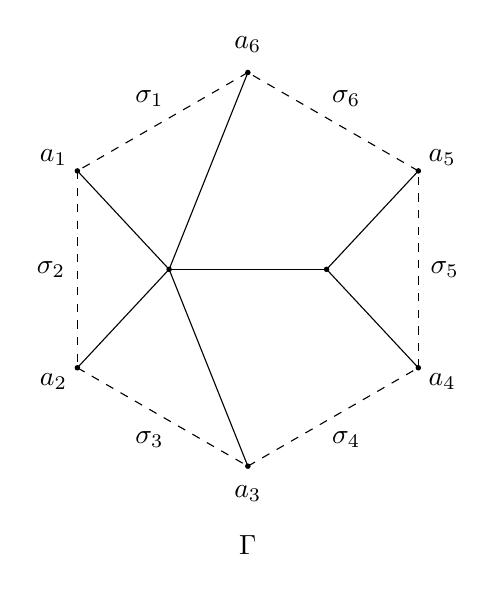
\begin{tikzpicture}
      \coordinate (b1) at (-1, 0);
      \coordinate (b2) at (1, 0);
      
      \fill (b1) circle (1pt);
      \fill (b2) circle (1pt);

      \foreach \i/\t in {1/60, 2/120, 3/180, 4/240, 5/300, 6/360} {
        \coordinate (a\i) at (\t+90:2.5);
        \fill (a\i) circle (1pt);
        \draw (a\i) [dashed]-- (\t+150:2.5);
        \node at (\t+90:2.85) {$a_{\i}$};
        \node at (\t+60:2.5) {$\sigma_{\i}$};
      }
      
      \draw (a6) -- (b1);
      \draw (a1) -- (b1);
      \draw (a2) -- (b1);
      \draw (a3) -- (b1);
      
      \draw (a4) -- (b2);
      \draw (a5) -- (b2);
      
      \draw (b1) -- (b2);

      \node at (0, -3.5) {$\Gamma$};
    \end{tikzpicture}
    \hspace{1in}
    \begin{tikzpicture}
      \foreach \i/\t in {1/60, 2/120, 3/180, 4/240, 5/300, 6/360} {
        \coordinate (a\i) at (\t+90:2.5);
        \fill (a\i) circle (1pt);
        \draw (a\i) [dashed]-- (\t+150:2.5);
        \node at (\t+90:2.85) {$a_{\i}$};
        \node at (\t+60:2.5) {$\sigma_{\i}$};
      }
      
      \coordinate (c11) at ($(b1)!0.45!(a6)$);
      \coordinate (c12) at ($(b1)!0.45!(a1)$);
      \coordinate (c13) at ($(b1)!0.45!(a2)$);
      \coordinate (c14) at ($(b1)!0.45!(a3)$);
      \coordinate (c15) at ($(b1)!0.45!(b2)$);
      
      \coordinate (c21) at ($(b2)!0.25!(b1)$);
      \coordinate (c22) at ($(b2)!0.45!(a4)$);
      \coordinate (c23) at ($(b2)!0.45!(a5)$);
      
      \foreach \i/\nsides in {1/5, 2/3} {
        \foreach \j in {1, 2, ..., \nsides} {
          \fill (c\i\j) circle (1pt);
        }
      }
      
      \foreach \i/\nsides in {1/5, 2/3} {
        \draw (c\i1)
        \foreach \j in {1, ..., \nsides} {
           -- (c\i\j)
        }
          -- cycle;
      }
      
      \draw (c11) -- (a6);
      \draw (c12) -- (a1);
      \draw (c13) -- (a2);
      \draw (c14) -- (a3);
      
      \draw (c21) -- (c15);
      
      \draw (c22) -- (a4);
      \draw (c23) -- (a5);
      
      \node at ($0.2*(c11) + 0.2*(c12) + 0.2*(c13) + 0.2*(c14) + 0.2*(c15)$) {$M$};
      \node at ($0.333*(c21) + 0.333*(c22) + 0.333*(c23)$) {$M$};
      
      \node at (0, -3.5) {$\Gamma_{{M}}$};
    \end{tikzpicture}}
    \caption{Example of $\Gamma \in \TSP\protect\p{\mathcal{P}_{\ba}}$ and its corresponding $M$-graph $\Gamma_{M}$.}\label{example}
  \end{figure}


\begin{definition}\label{M-graph-value-definition}
Given an $M$-graph \smash{$\Gamma_{M}$}, we assign a value to $\Gamma$ according to the following rule. For any $t\in[0,1)$ and $\bsig\in\{+,-\}^n$, we define the values of the edges in $\Gamma_{M}$ as follows. 
  \begin{enumerate}
    \item If $e = \p{a_k, b}$ is an external edge lying between regions $R_k$ and $R_{k+1}$, then we define
      \begin{equation}\label{f-external2}
        g_{t,\bsig}\p{e} := \Theta^{\p{\sig_{k}, \sig_{k+1}}}_{t}(a_k,b) \, .
      \end{equation}

    \item If $e = \p{b_1, b_2}$ is an internal unlabeled edge lying between regions $R_k$ and $R_{l}$, then we define
      \begin{equation}\label{f-internal2}
        g_{t,\bsig}\p{e}
          := \big(tS^{(\sB)}\Theta^{(\sig_k,\sig_{l})}_{t}\big)\p{b_1,b_2} .
      \end{equation}

    \item Corresponding to each loop of $M$-edges as in \eqref{eq:M-loopexample}, we define its value as 
  \begin{equation}\label{eq:Mloop_defgen}
    \cal F\p{b_i} \equiv W^{(k_i-1)d} \cal M_{\bsig(b_i),\ba(b_i)}^{(k_i)}, %=W^{-d} \avg{\prod_{j=1}^{k_i} \left[M\p{\sigma_j{(b_i)}}\id_{b_{i,j}}\right]},
  \end{equation}
 where we recall the $M$-loop defined in \eqref{eq:KMloop}. %and $\id_a:=W^dE_a$ is the block identity with.  
 Here, the charges $\sig_j(b_i)$ and vertices $a_j(b_i)$ are fixed according to the following rule: for each $j \in \qqq{k_i}$, the edge $\p{b_{i,j-1} \to b_{i,j}}$ (with the cyclic convention that $b_{i,0}=b_{i,k_i}$) belongs to exactly one region $R_{k_j}$. Then, we set ${\sigma}_j{\p{b_i}} = {\sigma}_{k_j}$ and $a_j{\p{b_i}} = b_{i,j}$. 
 
%  In simpler terms, $\cal F\p{b_i}$ is an $M$-loop that shares the same orientation as  $\mathcal{P}_{\ba}$, with each edge having the same color as the region it lies in. See \Cref{Fig2:charge-example} for an example of how to assign charges and directions to the $M$-loops.
    
    % If $e = \p{[b_1], [b_2]}$ is an internal $M$-edge belonging to the region $R_k$, then %we define
    %   \begin{equation}\label{f-internalM}
    %     g_{\bsig,z}\p{e}
    %       := m_t(z,\sig_k)\delta_{[b_1][b_2]}\, .
    %   \end{equation}
      
  \end{enumerate}
Now, we assign a value $\Gamma^{(n)}_{M;t,\bsig,\ba}$ to $\Gamma_M$ as:
\begin{equation}\label{M-graph-value-unsummed2}
\Gamma^{(n)}_{M;t,\bsig,\ba} := \sum_{b_{i,j} \in \Zn,\; i\in\qqq{r},\; j\in\qqq{k_i}}  \prod_{\text{unlabeled }e} g_{t,\bsig}(e) \cdot \prod_{i=1}^r \cal F(b_i) \,  ,
\end{equation}
where $b_{i,j}$'s denote the internal vertices in $\Gamma_M$ and $e$ denotes all unlabeled (i.e., non-$M$) edges.  
\end{definition}

It is straightforward to verify that the definition in \eqref{M-graph-value-unsummed2} is consistent with \eqref{M-graph-value-unsummed} in the case of random band matrices, where $M(\sig) = m(\sig) I$. Furthermore, in the block Anderson model, the tree representation formula \eqref{eq_Ktree} extends as follows.
 

\begin{lemma}[Lemma 4.16 of \cite{RBSO1D}]\label{tree-representation_BA}
In the setting of the block Anderson model, for any $n\ge 4$, $t\in[0,1)$, $\bsig\in \{+,-\}^n$, and $\ba\in (\Zn)^n$, we have the following representation formula for $\cal K$-loops:
\begin{equation}\label{eq:tree_rep2}
\cK_{t,\bsig,\ba}^{(n)}
=W^{-d(n-1)} \sum_{\Gamma \in \TSP\p{\mathcal{P}_{\ba}}} \Gamma^{(n)}_{M;t,\bsig,\ba}.
  \end{equation}
\end{lemma}

 

Next, we recall the molecule structure of $\mathcal{K}^{(n)}_{t,\bsig, \mathbf{a}}$ given in Section 3.3 of \cite{YY_25}. We split the $M$-graphs $\Gamma_M$ with $\Gamma\in \TSP(\mathcal{P}_{\mathbf{a}})$ according to which edges of the tree are ``long''---we refer to a \smash{$\Theta_t^{(\sig_1,\sig_2)}$}-edge as a \emph{long edge} if $\sig_1\ne \sig_2$, and a \emph{short edge} otherwise. We adopt this terminology because, according to \eqref{prop:ThfadC} and \eqref{prop:ThfadC_short}, the short edge decays on a scale of order 1, which is much shorter than the decay scale $\ell_t$ for a long edge. Given any $\bsig \in \{+, -\}^{n}$, define the subset of long internal edges (i.e., the boundary between two nontrivial neighbors of different charges) as 
\[
{\cal F}_{\mathrm{long}}(\Gamma, \bsig) := \left\{\{k,l\} \in \Z^{\mathrm{off}}_n: R_k\cap R_l\neq \emptyset ,\ \sigma_k\ne \sigma_l \right\},
\]
where we define the subset 
\[
\Z^{\mathrm{off}}_n :=\left\{\{k, l\} : 1 \leq k < l \leq n,\, k - l \pmod n \notin \{1,-1\}\right\}.
\]
Given any subset \(\pi \subset \mathbb{Z}_n^{\mathrm{off}}\), we use \(\TSP(\mathcal{P}_{\ba}, \bsig, \pi) := \big\{\Gamma \in \TSP(\mathcal{P}_{\ba}) : {\cal F}_{\text{long}}(\Gamma, \bsig) = \pi\big\}\) to denote the set of all $\Gamma$ such that \(\pi\) labels the pairs of all non-trivial neighbors in $\Gamma$ (note $\pi$ can be $\emptyset$). Then, we define 
  \begin{align}\label{eq:defKpi}
    \cK^{\p{\pi}}\p{t,\bsig,\ba}
      :=\sum_{\Gamma \in \TSP\p{\mathcal{P}_{\ba}, \bsig, \pi}} \Gamma^{\p{n}}_{M;t,\bsig,\ba}  .
  \end{align}
% (meaning that they are associated to $\Theta^{(B)}_{t|m|^2}$ as opposed to $\Theta^{(B)}_{tm^2}$ or $\Theta^{(B)}_{t\overline{m}^2}$). More precisely,
% \begin{equation*}
%     TSP(\mathcal{P}_{\mathbf{a}}) = \bigsqcup_{\pi\subset\Z^{off}_n} TSP(\mathcal{P}_{\mathbf{a}}, \bsig, \pi),
% \end{equation*}
% where $\Z^{off}_n$ is the set of pares of non-consecutive edges of $\mathcal{P}_{\mathbf{a}}$. See Definition 3.8 of \cite{YY_25} for the exact details. The key observation needed in this section is that the subsets $\pi\subset\Z^{off}_n$ encode the different ``molecule structures'' of trees $\Gamma_{\mathbf{a}}\in TSP(\mathcal{P}_{\mathbf{a}})$. 
Note that $\mathcal{K}^{(n)}_{t,\bsig, \mathbf{a}}$ can be decomposed as 
\begin{equation}\label{eq_K-Kpi}
    \mathcal{K}^{(n)}_{t, \bsig, \mathbf{a}} = W^{-d(n-1)}\sum_{\pi\subset \mathbb{Z}_n^{\rm{off}}} \mathcal{K}^{(\pi)}(t, \bsig, \mathbf{a}).
\end{equation}
Moreover, we have the following molecule decomposition of $\mathcal{K}^{(\pi)}$ given in equation (3.53) of \cite{YY_25}:
\begin{equation}\label{eq:molecule-Kpi}
    \mathcal{K}^{(\pi)}(t, \bsig, \mathbf{a}) = \sum_{\mathbf{b},\mathbf{c}} \prod_{k=1}^n \Theta^{(\sig_k,\sig_{k+1})}_{t,a_k b_k} \cdot \prod_{k=1}^{r-1} \left(tS^{(\sB)} \Theta_t^{(+,-)}\right)_{c_{2k-1} c_{2k}} \cdot \prod_{k=1}^r \Sigma^{(\pi)}(t, \bsig^{(k)}, \mathbf{b}^{(k)}).
\end{equation}
Here, each term $\Sigma^{(\pi)}(t, \bsig^{(k)}, \mathbf{b}^{(k)})$ represents a \emph{molecule}, defined as a maximal subgraph consisting solely of $M$-loops and \emph{short (unlabeled) internal edges}.\footnote{
With a slight abuse of notation, we again use the term ``molecule'' here. This definition is in the same spirit as that in \Cref{def_poly}, although the graph considered here is different from the one in \Cref{def_graph1}.
} 
In other words, if each molecule is collapsed into a single vertex, the resulting quotient graph contains only long internal edges connecting different molecules, along with external edges, which may be either short or long. 
In \eqref{eq:molecule-Kpi}, we assume there are $r$ molecules in total. The terms \smash{$tS^{(\sB)} \Theta_t^{(+,-)}$} correspond to the long internal edges $(c_{2k-1},c_{2k})$ between molecules, while the terms \smash{$\Theta^{(\sig_k,\sig_{k+1})}_{t,a_k b_k}$} correspond to the external edges $(a_k,b_k)$. The vectors $\mathbf b=(b_1,\ldots, b_n)$ and $\mathbf c=(c_1, c_2,\ldots, c_{2r-3},c_{2r-2})$ denote the internal vertices that serve as endpoints of these external and long internal edges, respectively. Furthermore, $\bsig^{(k)}$ and $ \mathbf{b}^{(k)}$ specify the charges and distinguished vertices associated with the $k$-th molecule. All other internal vertices within the molecules are implicitly summed over.

%Moreover, $\bsig^{(k)}$ and $ \mathbf{b}^{(k)}$ denote the charges and vertices associated with the $k$-th molecule, while all the other internal vertices in the molecules have been summed over. 


%The terms $\Sigma^{(\emptyset)}(t, \bsig^{(k)}, \mathbf{b}^{(k)})$ are ``molecule weights'', which consist of products of $\Theta^{(B)}_{tm^2}$ and $\Theta^{(B)}_{t\overline{m}^2}$ and, thus, exhibit exponential decay when $\max_{i,j} |b^{(k)}_i - b^{(k)}_j| \gg 1$. \medskip


Using the estimate \eqref{prop:ThfadC_short}, we can derive the following exponential decay estimate on ``pure loops'' where all charges are identical.


\begin{lemma}\label{lem_pureloop} 
For $\bsig \in \{+, -\}^n$ with $\sigma_1 = \sigma_2 = \cdots = \sigma_n$, there exist constants $c_n,C_n>0$ such that 
\begin{equation}\label{res_pureKes}
\left|\mathcal{K}^{(n)}_{t, \bsig, \mathbf{a}}\right|\le C_n W^{-d(n-1)} \exp\left(-c_n\max_{i,j}|a_i-a_j|\right).
\end{equation} 
\end{lemma}
\begin{proof}
% We follow the proof of Corollary 3.5 in \cite{YY_25}. We use the tree representation in \eqref{eq_Ktree} and the decomposition of the tree terms into sums from (3.6) of \cite{YY_25}:
% \begin{equation*}
%     \Gamma_{\mathbf{a}}(t,\bsig)=\sum_{\mathbf{b}\in(\Z_{L}^{2})^{n}}\Gamma^{(\mathbf{b})}_{\mathbf{a}}(t,\bsig),
% \end{equation*}
In the tree representation \eqref{eq:tree_rep2}, each term $\Gamma^{(n)}_{M;t,\bsig,\ba}$ on the RHS contains only $M$-edges and short unlabeled edges. Using the exponential decay from \eqref{prop:ThfadC_short}, along with the bound \eqref{Mbound_AO} or \eqref{Mbound_AO2} for $M$-edges in the setting of the block Anderson model, we obtain the desired estimate. 
% \begin{equation*}
%     |\Gamma^{(n)}_{t,\bsig,\ba}|\leq C_{n}\exp\left(-c_{n}\max_{i,j}|b_{i}-b_{j}|-c_{n}\max_{i,j}|a_{i}-b_{j}|\right).
% \end{equation*}
% Plugging this into the tree representation of $\mathcal{K}$ in \eqref{eq_Ktree}, completes the proof.
\end{proof}

We are now ready to prove the key bounds on $\cK$-loops, stated in \Cref{ML:Kbound}. The proof is analogous to that of Lemma 3.11 in \cite{YY_25}, but requires additional modifications to handle the higher-dimensional setting $d \ge 3$. For the reader's convenience, we provide the proof below.



% \begin{lemma}\label{ML:Kbound+pi}
% For any $\mathbf{a} \in \left(\Z_L^d\right)^n$ and $\bsig \in \left\{+, -\right\}^n$, we have the estimate
% \begin{equation}\label{eq:bcal_k_2}
%   \left|{\cal K}^{(n)}_{t, \bsig, \mathbf{a}}\right| \prec \left(W^{-d}B_{t,0}\right)^{n-1}.    
% \end{equation}
% \end{lemma}

\begin{proof}[\bf Proof of \Cref{ML:Kbound}]
For $n=1$ we have $\cK^{(1)}_{t,\bsig,\ba}=m(\sig_1)=\OO(1)$, and for $n\in\{2,3\}$ the bound follows from the explicit formulas \eqref{Kn2sol} and \eqref{Kn3sol} together with \eqref{prop:ThfadC} and, for $n=3$, \eqref{prop:ThfadC_short} (and \eqref{Mbound_AO} or \eqref{Mbound_AO2} for the $M$-loop in the block Anderson model). Indeed, the three charge pairs $(\sig_1,\sig_2)$, $(\sig_2,\sig_3)$, and $(\sig_3,\sig_1)$ in \eqref{Kn3sol} cannot all consist of different charges, so at least one of the three $\Theta$-propagators in \eqref{Kn3sol} is short-range by \eqref{prop:ThfadC_short}, and its sum over the free index is $\OO(1)$ rather than $(1-t)^{-1}$; the other two propagators are bounded pointwise by $\OO(B_{t,0})$ using \eqref{prop:ThfadC}. This gives $|\cK^{(3)}_{t,\bsig,\ba}|\lesssim (W^{-d}B_{t,0})^2$. We may therefore assume $n\ge 4$, which is the range in which the tree representation \eqref{eq_Ktree} is available.
By \eqref{eq_K-Kpi}, it suffices to show that for any $\pi \subset \Z^{\rm{off}}_n$, we have
\begin{equation}\label{eq:K-pi-bound}
    \left|\mathcal{K}^{(\pi)}(t, \bsig, \mathbf{a})\right| \prec B_{t,0}^{n-1}.
\end{equation}
We prove the above bound by induction on the number of molecules $r$ in $\pi$. In order to carry out the induction step, we will prove \eqref{eq:K-pi-bound} for a slightly generalized quantity $\tilde{\mathcal{K}}^{(\pi)}$, defined by
\begin{equation}\label{eq:wtKpi}
    \tilde{\mathcal{K}}^{(\pi)}(t, \bsig, \mathbf{a}) = \sum_{\mathbf{b},\mathbf{c}} \prod_{k=1}^n \tilde{\Theta}_{t,a_k b_k} \cdot \prod_{k=1}^{r-1} \left(tS^{(\sB)}\Theta^{(+,-)}_{t}\right)_{c_{2k-1} c_{2k}} \cdot \prod_{k=1}^r \Sigma^{(\pi)}(t, \bsig^{(k)}, \mathbf{b}^{(k)}),
\end{equation}
where each $\tilde{\Theta}_{t}$ represents either $\Theta^{(\sig,\sig')}_{t}$ for some $\sig,\sig'\in\{+,-\}$ or $tS^{(\sB)}\Theta^{(+,-)}_{t}$.  

We start with the single molecule case with $\pi=\emptyset$. In this case, we can write 
\begin{equation*}
    \tilde{\mathcal{K}}^{(\emptyset)}(t, \bsig, \mathbf{a}) = \sum_{\mathbf{b}} \prod_{i=1}^n \tilde{\Theta}_{t,a_i b_i} \cdot \Sigma^{(\emptyset)}(t, \bsig, \mathbf{b}).
\end{equation*}
First, the $M$-edges and short unlabeled edges in $\tilde{\mathcal{K}}$, including all edges contained within the molecule,
% have weights \smash{$\Theta^{(\sB)}_{tm^2}$}, \smash{$\Theta^{(\sB)}_{tm^2} - I$}, \smash{$\Theta^{(\sB)}_{t\bar{m}^2}$}, or \smash{$\Theta^{(\sB)}_{t\bar{m}^2} - I$}, which 
have constant size and fast exponential decay outside their constant range by \eqref{prop:ThfadC_short}, together with \eqref{Mbound_AO} or \eqref{Mbound_AO2} in the block Anderson model. Thus, the molecule $\Sigma^{(\emptyset)}$ has constant size and fast exponential decay as well:
\begin{equation}\label{eq:molecule-decay}
    \left|\Sigma^{(\emptyset)}(t, \bsig, \mathbf{b})\right| \le C\exp\left\{-c\max_{i,j} |b_i-b_j|\right\}
\end{equation}
for some constants $c,C>0$. Additionally, if we have a pure loop (i.e., $\bsig$ consists entirely of the same charge), then every edge in $\tilde{\mathcal{K}}^{(\emptyset)}$ is short, so we have 
\begin{equation*}
    \left|\tilde{\mathcal{K}}^{(\emptyset)}(t, \bsig, \mathbf{a})\right| \le C\exp\left\{-c\max_{i,j} |a_i-a_j|\right\} \lesssim B_{t,0}^{n-1}.
\end{equation*}
If $\bsig$ is not a pure loop, then without loss of generality, we can assume that $\sigma_1 \neq \sigma_2$. In this case, we have 
\begin{equation*}
    \tilde{\mathcal{K}}^{(\emptyset)}(t, \bsig, \mathbf{a}) = \sum_{b_1} \tilde{\Theta}_{t,a_1b_1} \sum_{\mathbf{b}\setminus \{b_1\}} \Sigma^{(\emptyset)}(t, \bsig, \mathbf{b}) \prod_{i=2}^n  \tilde{\Theta}_{t,a_i b_i}.
\end{equation*}
We now claim that 
\begin{equation}\label{eq:ind-step-bound}
    \sum_{b_1} \bigg|\sum_{\mathbf{b}\setminus \{b_1\}} \Sigma^{(\emptyset)}(t, \bsig, \mathbf{b}) \prod_{i=2}^n \tilde{\Theta}_{t,a_i b_i}\bigg| \prec B_{t,0}^{n-2}.
\end{equation}
Combining this estimate with the bound \eqref{prop:ThfadC} for the $\Theta$-propagators, we obtain that 
\begin{align*}
    \left|\tilde{\mathcal{K}}^{(\emptyset)}(t, \bsig, \mathbf{a})\right| %&\le \sum_{b_1} \left(\tilde{\Theta}^{(sB)}_{t}\right)_{a_1b_1} \bigg|\sum_{\mathbf{b}\setminus \{b_1\}} \Sigma^{(\emptyset)}(t, \bsig, \mathbf{b}) \prod_{i=2}^n \left(\tilde{\Theta}^{(\sB)}_{tm_i m_{i+1}}\right)_{a_i b_i}\bigg| \\
    &\lesssim B_{t,0}\sum_{b_1} \bigg|\sum_{\mathbf{b}\setminus \{b_1\}} \Sigma^{(\emptyset)}(t, \bsig, \mathbf{b}) \prod_{i=2}^n \tilde{\Theta}_{t,a_i b_i}\bigg| \prec B_{t,0}^{n-1}.
\end{align*}
This concludes \eqref{eq:K-pi-bound} for the case $\pi=\emptyset$.


To prove the bound \eqref{eq:ind-step-bound}, we consider two cases depending on whether (i) $\bsig$ is non-alternating, or (ii) $\bsig$ is alternating, where $\sig_j\ne \sig_{j+1}$ for all $j\in \qqq{n}$.  

\medskip
{\noindent\bf (i)} If $\bsig$ is non-alternating, then there exists $j\in\qqq{2,n}$ such that $\sigma_j = \sigma_{j+1}$. The corresponding short edge has fast exponential decay on the constant scale by \eqref{prop:ThfadC_short}: % and \eqref{Mbound_AO} or \eqref{Mbound_AO2}:
\begin{equation}\label{eq:shortexternal}
    \left|\tilde{\Theta}_{t,a_jb_j}\right| \le C\exp\{-c|a_j - b_j|\}.
\end{equation}
For the remaining $(n-2)$ factors \smash{$\tilde{\Theta}_{t,a_i b_i}$}, we can bound them pointwise using \eqref{prop:ThfadC} as
\be\label{eq:pointwise_Theta}
    \left|\tilde{\Theta}_{t,a_ib_i}\right| \lesssim B_{t,0}, \quad \forall i \in\qqq{2,n} \setminus \{j\}.
\ee
The above two bounds, together with the exponential decay for the molecule weight in \eqref{eq:molecule-decay}, allow us to bound the summation on the LHS of \eqref{eq:ind-step-bound} by $B_{t,0}^{n-2}$. % which gives \eqref{eq:ind-step-bound} in the non-alternating case.

 

\medskip
{\noindent\bf (ii)} It remains to handle the challenging case of alternating $\bsig$. In this setting, in addition to the constant-range exponential decay, we must also use the sum-zero property of molecule weights:
\begin{equation}\label{eq:Sigma-empty-sum-zero}
    \sum_{\mathbf{b}\setminus \{b_1\}} \Sigma^{(\emptyset)}(t, \bsig, \mathbf{b}) = \OO(|1-t|),\quad \sum_{\mathbf{b}\setminus \{b_1\}} \big|\Sigma^{(\emptyset)}(t, \bsig, \mathbf{b})\big| = \OO(\ilambda^2+|1-t|).
\end{equation}
The first estimate was established in \cite[Lemma 3.10]{YY_25} for 1D random band matrices and in \cite[Lemma 4.29]{RBSO1D} for 1D and 2D block Anderson models, while the second estimate was proved in \cite[Claim 4.30]{RBSO1D}. Importantly, these proofs are dimension-independent: they rely only on the pure loop estimate (\Cref{lem_pureloop}), the short-edge bound \eqref{prop:ThfadC_short}, the $M$-edge bound \eqref{Mbound_AO} or \eqref{Mbound_AO2}, and Ward's identity \eqref{WI_calK} for $\cal K$-loops.


We now decompose the long external edges into three parts as follows:
\begin{align*}
\tilde{\Theta}^{(+,-)}_{t,a_jb_j} = f_0(a_j, s_j) + f_1(a_j, s_j) + f_2(a_j, s_j), \quad \tilde{\Theta}_{t}^{(+,-)}\in \big\{\Theta^{(+,-)}_{t},\ tS^{(\sB)}\Theta^{(+,-)}_{t}\big\}  ,
\end{align*}
where we denote $f(a_j, s_j)= \tilde{\Theta}^{(+,-)}_{t}\p{a_j,b_1+s_j}$ with $s_j = b_j - b_1$, and 
\begin{align*}
    %f(a_j, s_j) &= \big(\tilde{\Theta}^{(\sB)}_{t}\big)_{a_j,b_1+s_j},\\
    f_0(a_j, s_j) &= f(a_j, 0),\quad
    f_1(a_j, s_j) = \frac12 f(a_j, s_j) - \frac12 f(a_j, -s_j),\\
    f_2(a_j, s_j) &= \frac12 f(a_j, s_j) + \frac12 f(a_j, -s_j) - f(a_j, 0).
\end{align*}
By \Cref{lem_propTH}, we have the following bounds under the condition $|s_j|\prec 1$ for $j\in\qqq{2,n}$ (if $|a_j-b_1|\ge 4|s_j|$, the bounds on $f_1$ and $f_2$ follow from \eqref{prop:BD1} and \eqref{prop:BD2} with $c_0=1/2$, recalling that $S^{(\sB)}$ has range $1$; otherwise, $|a_j-b_1|<4|s_j|\prec 1$, and they follow from \eqref{prop:ThfadC0}, since the zero mode cancels in $f_1$ and $f_2$):
\begin{align}\label{eq:f12}
    \left|f_0(a_j, s_j)\right| &\lesssim B_{t,|a_j - b_1|} \le B_{t, 0},\quad \left|f_1(a_j, s_j)\right| \prec \frac{(\ilambda^2+|1-t|)^{-1}}{|a_j - b_1|^{d-1}+1},\quad 
    \left|f_2(a_j, s_j)\right| \prec \frac{(\ilambda^2+|1-t|)^{-1}}{|a_j - b_1|^{d}+1}.
\end{align}
We view $\Sigma^{(\emptyset)}(t, \bsig, \mathbf{b}) = g(\mathbf{s})$ as a function of the shifts $\mathbf{s} = (s_2, \ldots, s_n)$. Then, we can write 
\begin{equation*}
    \sum_{\mathbf{b}\setminus \{b_1\}} \Sigma^{(\emptyset)}(t, \bsig, \mathbf{b}) \prod_{j=2}^n \tilde{\Theta}_{t,a_j b_j} = \sum_{\mathbf{s}} g(\mathbf{s}) \prod_{j=2}^n \sum_{\xi_j\in\{0,1,2\}} f_{\xi_j}(a_j, s_j).
\end{equation*}
We split the sum above into several parts.
\begin{enumerate}

    \item Consider the terms where $\xi_j = 0$ for all $j\in\qqq{2,n}$. Then, we use the sum-zero property \eqref{eq:Sigma-empty-sum-zero} to get 
    \begin{align*}
        \sum_{b_1}\bigg|\sum_{\mathbf{s}} g(\mathbf{s}) \prod_{j=2}^n f_{0}(a_j, s_j)\bigg| &\lesssim (1-t)\sum_{b_1}\prod_{j=2}^n \left|\tilde{\Theta}_{t,a_jb_1}\right|\lesssim (1-t) B_{t, 0}^{n-2} \sum_{b_1} \left|\tilde{\Theta}_{t,a_2b_1}\right| \lesssim B_{t, 0}^{n-2},
    \end{align*}
    where in the second step, we use \eqref{eq:pointwise_Theta} for all but one $\tilde{\Theta}_{t}$ factor, and in the last step, we use \eqref{eq:THETAinftinf}. 

    \item Consider the case where exactly one $\xi_j$ equals $1$ while all other $\xi_j$'s are zero. In this situation, the sum vanishes by the skew symmetry of $f_1$ (namely, $f_1(a_j, s_j) = -f_1(a_j, -s_j)$) together with the symmetry of $\Sigma^{(\emptyset)}$ (i.e., $g(\mathbf{s}) = g(-\mathbf{s})$). The latter symmetry follows from the translation invariance and symmetry of the $\Theta$-propagators (\Cref{lem_propTH}) and of the $M$-loops (\Cref{lem:propM}).
    
    \item Suppose there is at least one $i\in\qqq{2,n}$ such that $\xi_i = 2$. Then, using \eqref{eq:f12} and \eqref{eq:Sigma-empty-sum-zero}, we get 
    \begin{equation*}
     \qquad   \sum_{b_1}\bigg|\sum_{\mathbf{s}} g(\mathbf{s}) f_2(a_i, s_i) \prod_{j\notin \{1,i\}} f_{\xi_j}(a_j, s_j)\bigg| \prec \frac{B_{t, 0 }^{n-2}}{\ilambda^2+|1-t|} \sum_{b_1} \frac{1}{|a_i-b_1|^{d}+1} \sum_{\mathbf{b}\setminus \{b_1\}} \big|\Sigma^{(\emptyset)}(t, \bsig, \mathbf{b})\big| \prec B_{t, 0 }^{n-2}.
    \end{equation*}

    \item Suppose there are at least two $i,k\in \qqq{2,n}$ such that $i\neq k$ and $\xi_i=\xi_k = 1$. In this case, using \eqref{eq:f12} and \eqref{eq:Sigma-empty-sum-zero}, we get 
    \begin{align*}
     \quad   \sum_{b_1}\bigg|\sum_{\mathbf{s}} g(\mathbf{s}) f_1(a_i, s_i) f_1(a_k, s_k)\prod_{j\notin \{1,i,k\}} f_{\xi_j}(a_j, s_j)\bigg| \prec \frac{B_{t, 0 }^{n-3}}{\ilambda^2+|1-t|} \sum_{b_1} \frac{1}{|a_i-b_1|^{d-1}+1}\frac{1}{|a_k-b_1|^{d-1}+1} \\
        \lesssim  B_{t, 0 }^{n-2}  \sum_{b_1} \left[\frac{1}{|a_i-b_1|^{d}+1}\frac{1}{|a_k-b_1|^{d-2}+1}+\frac{1}{|a_i-b_1|^{d-2}+1}\frac{1}{|a_k-b_1|^{d}+1}\right] \lesssim B_{t, 0 }^{n-2},
        % \\&
        % \lesssim B_{t, 0 }^{n-2} \sum_{b_1} \left[\frac{1}{|a_i-b_1|^{d}+1}+\frac{1}{|a_k-b_1|^{d}+1}\right] \prec B_{t, 0 }^{n-2},
    \end{align*}
    where, in the second step, we also use $(\ilambda^2+|1-t|)^{-1}\lesssim B_{t,0}$ and the elementary inequality
    \[\frac{1}{(x^{d-1}+1)(y^{d-1}+1)}\le 2\left[\frac{1}{(x^{d}+1)(y^{d-2}+1)}+\frac{1}{(x^{d-2}+1)(y^{d}+1)}\right],\qquad \forall\, x,y\ge 0 .\]
    This asymmetric splitting is the modification of the argument in \cite[Lemma 3.11]{YY_25} needed for $d\ge 3$: since $d-2\ge 1$, each of the two resulting lattice sums over $b_1$ in the second line is $\OO(1)$, uniformly in $a_i$, $a_k$, and $L$. 

\end{enumerate}
This concludes the proof of the claim \eqref{eq:ind-step-bound}. 
% Now to finish the case $\pi=\emptyset$, we use \eqref{eq:ind-step-bound} to compute
% \begin{align*}
%     \left|\tilde{\mathcal{K}}^{(\emptyset)}(t, \bsig, \mathbf{a})\right| &\le \sum_{b_1} \left(\tilde{\Theta}^{(\sB)}_{t|m|^2}\right)_{a_1b_1} \left|\sum_{\mathbf{b}\setminus b_1} \Sigma^{(\emptyset)}(t, \bsig, \mathbf{b}) \prod_{i=2}^n \left(\tilde{\Theta}^{(\sB)}_{tm_i m_{i+1}}\right)_{a_i b_i}\right| \\
%     &\prec B_{t,0}\sum_{b_1} \left|\sum_{\mathbf{b}\setminus b_1} \Sigma^{(\emptyset)}(t, \bsig, \mathbf{b}) \prod_{i=2}^n \left(\tilde{\Theta}^{(\sB)}_{tm_i m_{i+1}}\right)_{a_i b_i}\right| \prec B_{t,0}^{n-1}.
% \end{align*}


Finally, we establish \eqref{eq:K-pi-bound} by induction on the number of molecules $r$. 
Assume that \eqref{eq:K-pi-bound} holds for every $\pi$ with at most $n$ external vertices and at most $(r-1)$ molecules. 
%Suppose that \eqref{eq:K-pi-bound} holds for any $\pi$ with $\le n$ external vertices and $\le r-1$ molecules. 
Now, consider a configuration $\pi$ consisting of $r$ molecules. In the molecule-level quotient graph---where each molecule is represented as a single vertex---the molecules, together with the long internal edges, form a tree. Therefore, there exists a leaf in this tree. Without loss of generality, assume that the molecule indexed by $k=1$ in \eqref{eq:molecule-Kpi} is such a leaf, and that it is connected to $ a_1, \ldots, a_{l}$ by external edges. 
%Consider any $\pi$ with $r$ molecules. Note that in the molecule-level quotient graph, where each molecule is collapsed into a single vertex, the molecules together with the long internal edges form a tree, so there exists a leaf of this tree. Without loss of generality, assume that the molecule indexed by $k=1$ in \eqref{eq:molecule-Kpi} is a leaf and that it is connected to $a_1, \ldots, a_l$ by the external edges. 
Then, we can decompose \smash{$\tilde{\mathcal{K}}^{(\pi)}$} in \eqref{eq:wtKpi} as  
\begin{align}
    \left|\tilde{\mathcal{K}}^{(\pi)}(t, \bsig, \mathbf{a})\right| &= \bigg|\sum_{\mathbf{b}^{(1)}} \prod_{i=1}^l \tilde{\Theta}_{t,a_i b_i} \cdot \Sigma^{(\emptyset)}(t, \bsig^{(1)}, \mathbf{b}^{(1)}) \cdot\tilde{\mathcal{K}}^{(\pi')}(t, \bsig', \mathbf{a}')\bigg| \nonumber\\
    &\le \sum_{c_1}\bigg|\sum_{\mathbf{b}^{(1)}\setminus \{c_1\}} \prod_{i=1}^l \tilde{\Theta}_{t,a_i b_i} \cdot \Sigma^{(\emptyset)}(t, \bsig^{(1)}, \mathbf{b}^{(1)})\bigg| \cdot\left|\tilde{\mathcal{K}}^{(\pi')}(t, \bsig', \mathbf{a}')\right|, \label{eq:Kpipi}
\end{align}
where $\pi'$ consists of the remaining $(r-1)$ molecules, $\mathbf{b}^{(1)} = (b_1,\ldots, b_l,c_1)$ with $c_1$ denoting the vertex in the first molecule that connects to other molecules through a long internal edge, $\bsig^{(1)}=(\sig_1,\ldots,\sig_l,\sig_{l+1})$, $\mathbf{a}' = (c_1, a_{l+1}, \ldots, a_{n})$, and $\bsig' = (\sigma_{l+1}, \ldots, \sigma_n,\sig_1)$.  
Applying the induction hypothesis to bound \smash{$\tilde{\mathcal{K}}^{(\pi')}$}, and using \eqref{eq:ind-step-bound} to estimate the remaining part of the product (noting that \eqref{eq:ind-step-bound} is applicable because $\sigma_1 \neq \sigma_{l+1}$ by the definition of a molecule), we obtain that 
\begin{equation*}
    \left|\tilde{\mathcal{K}}^{(\pi)}(t, \bsig, \mathbf{a})\right| \prec B_{t, 0}^{l-1} \cdot B_{t, 0}^{n-l} = B_{t, 0}^{n-1}.
\end{equation*}
This concludes the proof of \Cref{ML:Kbound}.
\end{proof}

Finally, \Cref{lem_wardineq_K} follows from the bound \eqref{eq:ind-step-bound}, together with an induction argument analogous to the one used above in the proof of \Cref{ML:Kbound}.

\begin{proof}[\bf Proof of \Cref{lem_wardineq_K}]
By \eqref{eq_K-Kpi}, it suffices to prove that for any $\pi \subset \Z^{\rm{off}}_n$, 
\begin{equation}\label{eq:K-pi-bound_partial}
 \sum_{a_n}   \left|\mathcal{K}^{(\pi)}(t, \bsig, \mathbf{a})\right| \prec \eta_t^{-1}B_{t,0}^{n-2}.
\end{equation}
In the case $\pi=\emptyset$, using \eqref{eq:THETAinftinf} and \eqref{eq:ind-step-bound}, we can bound the LHS of \eqref{eq:K-pi-bound_partial} by 
\begin{equation}\nonumber
 \sum_{b_n} \sum_{a_n}\Theta^{(+,-)}_{t,a_n b_n} \bigg|\sum_{\mathbf{b}\setminus \{b_n\}} \Sigma^{(\pi)}(t, \bsig, \mathbf{b}) \prod_{i=1}^{n-1} \tilde{\Theta}_{t,a_i b_i}\bigg| \le \frac{1}{1-t}\sum_{b_n} \bigg|\sum_{\mathbf{b}\setminus \{b_n\}} \Sigma^{(\pi)}(t, \bsig, \mathbf{b}) \prod_{i=1}^{n-1} \tilde{\Theta}_{t,a_i b_i}\bigg| \prec \eta_t^{-1}B_{t,0}^{n-2}.
\end{equation} 
Here, in the last step, we have used that the external edge at $a_n$ is $\Theta^{(\sig_n,\sig_1)}_t$ with $\sig_n\ne\sig_1$, so that \eqref{eq:ind-step-bound} applies with $b_n$ playing the role of $b_1$. If $\sig_n=\sig_1$, this edge is short-range, and \eqref{prop:ThfadC_short} gives $\sum_{a_n}|\Theta^{(\sig_n,\sig_1)}_{t,a_nb_n}|=\OO(1)$. Then, bounding all but one of the remaining external edges pointwise as in \eqref{eq:pointwise_Theta}, summing the last one using \eqref{eq:THETAinftinf}, and summing over the other vertices of the molecule using \eqref{eq:molecule-decay}, we obtain the bound $\OO\big((1-t)^{-1}B_{t,0}^{n-2}\big)\lesssim\eta_t^{-1}B_{t,0}^{n-2}$ in this case as well. 
For $\pi\ne \emptyset$, we argue by induction as in the proof of \Cref{ML:Kbound}.
Assume that \eqref{eq:K-pi-bound_partial} holds for any $\pi$ with at most $n$ external vertices and at most $(r-1)$ molecules. Using the notation of \eqref{eq:Kpipi}, and applying \eqref{eq:ind-step-bound} together with the induction hypothesis, we obtain
\begin{align*}
\sum_{a_n} \left|\tilde{\mathcal{K}}^{(\pi)}(t, \bsig, \mathbf{a})\right| &\le \sum_{c_1}\bigg|\sum_{\mathbf{b}^{(1)}\setminus \{c_1\}} \prod_{i=1}^l \tilde{\Theta}_{t,a_i b_i} \cdot \Sigma^{(\emptyset)}(t, \bsig^{(1)}, \mathbf{b}^{(1)})\bigg| \cdot \sum_{a_n}\left|\tilde{\mathcal{K}}^{(\pi')}(t, \bsig', \mathbf{a}')\right| \\
&\prec B_{t, 0}^{l-1} \cdot \eta_t^{-1}B_{t, 0}^{n-l-1} =\eta_t^{-1} B_{t, 0}^{n-2}. 
\end{align*}
This concludes the proof of \eqref{eq:K-pi-bound_partial}.
\end{proof}













